\chapter{Diseño e Implementación}
\label{cap:capitulo4}

El objetivo de este \ac{TFG} es desarrollar un sistema de conducción autónoma capaz de realizar un seguimiento de carril, control de crucero adaptativo y maniobras de adelantamiento completas de forma segura en un entorno simulado. En este capítulo, se establecen primero los fundamentos de la percepción, definiendo qué elementos del entorno pueden ser detectados y qué información estará disponible para los modelos de toma de decisiones. A continuación, se explica el sistema implementado de conducción autónoma tradicional basado en el seguimiento de carril mediante un controlador \ac{PID}. Posteriormente, se exploran algoritmos basados en \ac{DRL} aplicados a la conducción autónoma, desarrollando y evaluando distintos modelos para la generación de comportamientos inteligentes. Finalmente, se lleva a cabo un análisis comparativo de los diferentes enfoques implementados, destacando sus ventajas e inconvenientes en el contexto de la conducción autónoma en un escenario urbano.

\section{Arquitectura general}

A continuación, se detalla la arquitectura general del sistema, ilustrada en la Figura \ref{fig:arch}, que consta de tres módulos principales. El vehículo en CARLA incluye los sensores y actuadores que permiten al sistema interactuar con el entorno. Entre los sensores, el sistema dispone de cámaras RGB y \ac{LiDAR}, mientras que los actuadores cuentan con acelerador y giro. La información captada por los sensores se transfiere al módulo de percepción para su procesamiento inteligente, cuyo objetivo es extraer información relevante y simplificada, que servirá como observaciones para los modelos de conducción autónoma. La cámara RGB permite la detección del carril y de la calzada, mientras que el \ac{LiDAR} posibilita la detección de otros vehículos en la carretera. Finalmente, con este post-procesado, el módulo de toma de decisiones es capaz de conseguir diferentes comportamientos autónomos basados en diversos algoritmos. Estas decisiones se aplican directamente en los actuadores del vehículo CARLA.

\begin{figure}[ht]
  \centering
  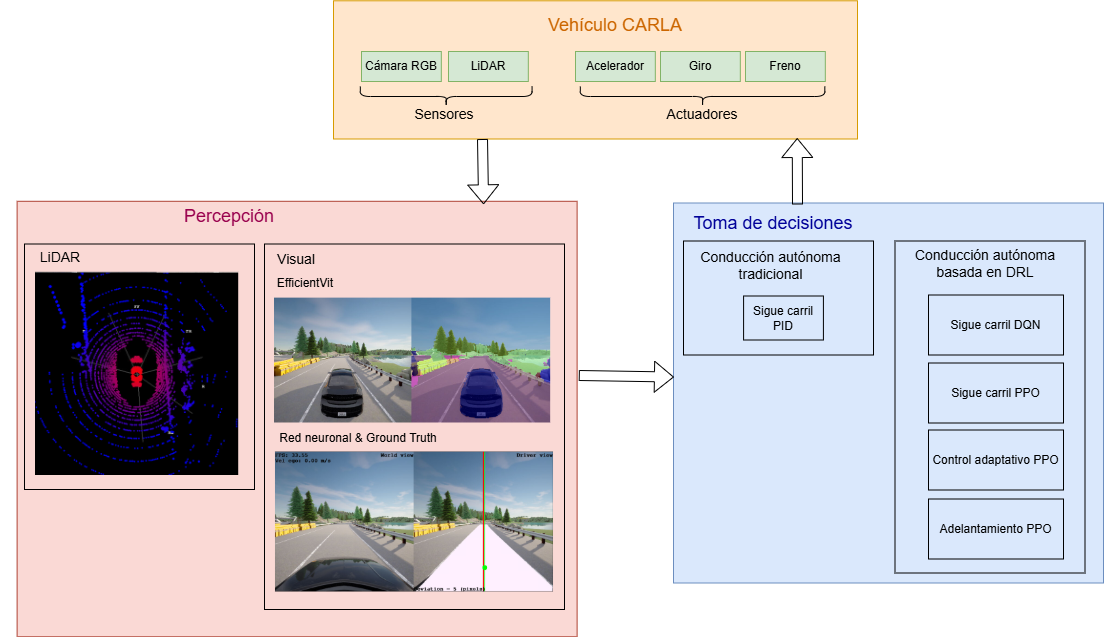
\includegraphics[width=16cm]{figs/Diseño/arquitectura.png}
  \caption{Arquitectura general.}
  \label{fig:arch}
\end{figure}

\section{Percepción visual}

La percepción visual es esencial para entender el entorno y tomar decisiones informadas en un sistema de conducción autónoma. Una habilidad básica de este tipo de sistema es la detección del carril que debe seguir. Para ir aún más allá, también se ha añadido un submódulo capaz de segmentar la calzada, lo que, por ejemplo, permite al sistema comprobar la existencia de otros carriles.

Las imágenes captadas por la cámara RGB del simulador CARLA tiene una resolución de 512 x 512 píxeles con un campo de visión de 90º, obteniendo imágenes detalladas con una perspectiva amplia. Esta cámara se coloca con una localización similar a la de un conductor. En esta sección, veremos cómo a partir de esta información y aplicando diversas herramientas, es posible identificar el carril y segmentar la imagen.

\subsection{Detección del carril}

La detección del carril por el que debe circular nuestro vehículo autónomo es fundamental para la toma de decisiones eficientes y seguras, garantizando que no se desvíe a otros carriles o fuera de los límites de la carretera. En esta sección, se analizan las fortalezas y debilidades de distintas técnicas de detección de carril: una perfecta basada en información de CARLA (\textit{ground truth}) y otra más realista basada en un modelo de \ac{DL}.

\subsubsection{Modelo basado en DL}

El modelo basado en \ac{DL} para la detección de carril, expuesto es la sección \ref{sec:carril_dl3}, procesa imágenes de 512 x 1024 píxeles, mientras que las nuestras son de 512 x 512 píxeles. Por ello, primero creamos una imagen vacía y colocamos la imagen capturada por la cámara RGB en el centro. Esta imagen se pasa como entrada al modelo, el cual devuelve dos máscaras de segmentación que definen las líneas del carril. En algunas situaciones, las líneas del carril pueden ser discontinuas o incompletas. Por ello, aplicamos un proceso de post-procesado para mejorar la detección y obtener una línea continua en toda la imagen sin importar las condiciones. Para lograrlo, aplicamos una regresión lineal a los puntos detectados de cada línea del carril. Este procedimiento nos permite calcular los coeficientes de las rectas que mejor se ajustan a esos puntos. Además, antes de aplicar la regresión lineal, se han aplicado técnicas de eliminación \textit{outliers} basadas en las medidas anteriores para lograr una detección aún más precisa del carril. 

Una vez tenemos los coeficientes de las rectas que definen cada línea del carril, es muy sencillo calcular la coordenada \textit{x} de cada punto de la línea dada la altura. Se ha definido una altura máxima para la detección del carril, creando así la forma de un trapecio, como se puede observar en la Figura \ref{fig:dl_final_carril}. Al unir los puntos a la misma altura, podemos obtener el área del carril, su centro de masas y la desviación del coche con respecto al carril, considerando el centro de la imagen como el centro de nuestro vehículo. Además, podemos calcular \textit{n} puntos de cada línea del carril igualmente espaciados en el eje \textit{y} para terminar de conformar la representación simplificada de carril que, posteriormente, podrán recibir los modelos para la toma de decisiones.

\begin{figure}[ht]
\centering
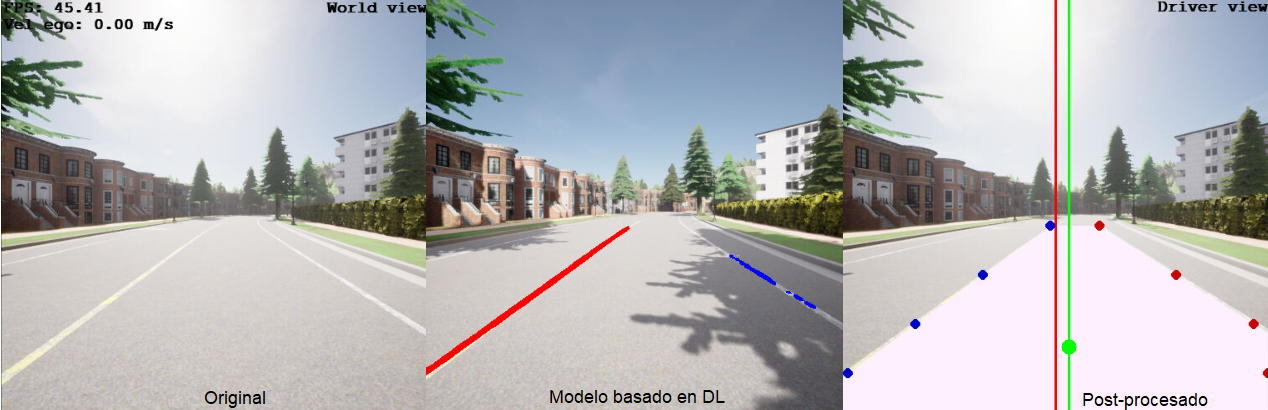
\includegraphics[width=14cm]{figs/Diseño/lane/lane_dl.png}
\caption{Detección de carril basada en \ac{DL}.}
\label{fig:dl_final_carril}
\end{figure}

También se ha implementado un sistema de memoria para filtrar mediciones erróneas. Este sistema almacena las cinco últimas detecciones de las líneas, junto con el ángulo que cada una forma con la horizontal. Si el ángulo de la detección actual difiere lo suficiente de la media de los ángulos almacenados o si no se detecta ninguna línea, descartamos la medida y utilizamos la última detección válida. Si esto ocurre durante más de cinco iteraciones consecutivas, determinamos que se ha perdido el carril.

Gracias al post-procesado aplicado, aunque el modelo basado en \ac{DL} no sea capaz de detectar completamente las líneas del carril, esta solución hace que sea eficiente en la mayoría de situaciones. A excepción de escenarios muy concretos donde hay un vehículo que obstruye la visibilidad de las líneas del carril, como se ve en la Figura \ref{fig:dl_final_carril_obs}. La única forma de mitigar este problema es reentrenar el modelo con un \textit{dataset} más amplio. Sin embargo, dado que este \ac{TFG} está enfocado en generar comportamientos de toma de decisiones y reentrenar el modelo requería tiempo y la generación de nuevos \textit{datasets}, se optó por emplear la técnica de \textit{ground truth}.
\begin{figure}[ht]
\centering
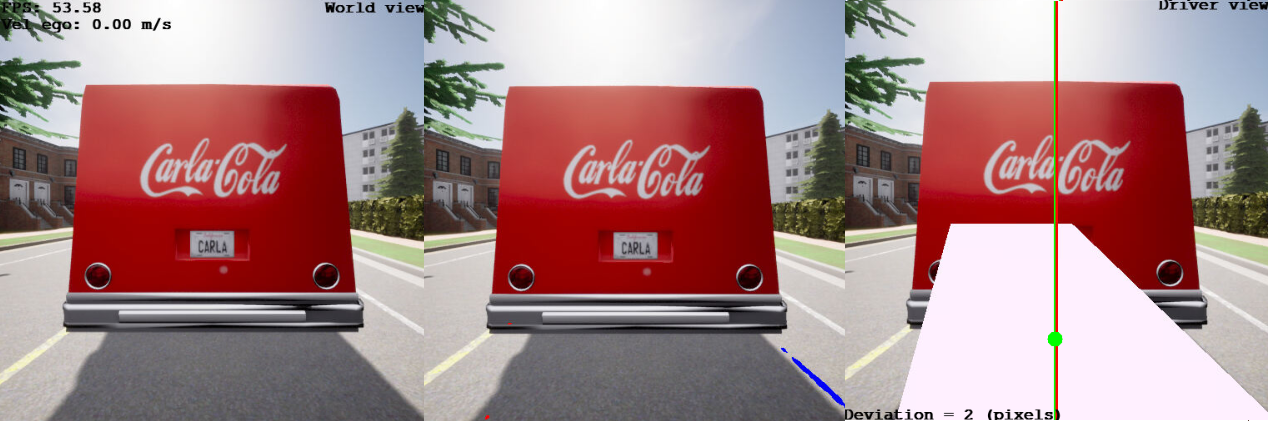
\includegraphics[width=14cm]{figs/Diseño/lane/lane_dl_obs.png}
\caption{Limitaciones de la detección de carril basada en \ac{DL}.}
\label{fig:dl_final_carril_obs}
\end{figure}

\subsubsection{Ground truth}

Si deseamos interactuar con otros vehículos en la carretera el modelo de detección de carril basado en \ac{DL} actual no es viable. Por esta razón, surge la necesidad de utilizar \textit{ground thruth} para asegurar una detección del carril fiable en cualquier tipo de situación, incluso cuando la visibilidad es limitada.

Una vez aplicada la técnica de \textit{ground thruth}, descrita en la sección \ref{sec:gt}, obtenemos algunos puntos de la línea del carril, pero no todos. Para completar esta información, utilizamos la función \textit{pygame.draw.lines}, que, a partir de este conjunto de puntos, reconstruye con precisión las líneas completas del carril. Posteriormente, aplicamos un proceso de post-procesado similar al anterior para determinar los límites de cada línea del carril en cada altura, permitiéndonos calcular sus métricas.

\begin{figure}[ht]
\centering
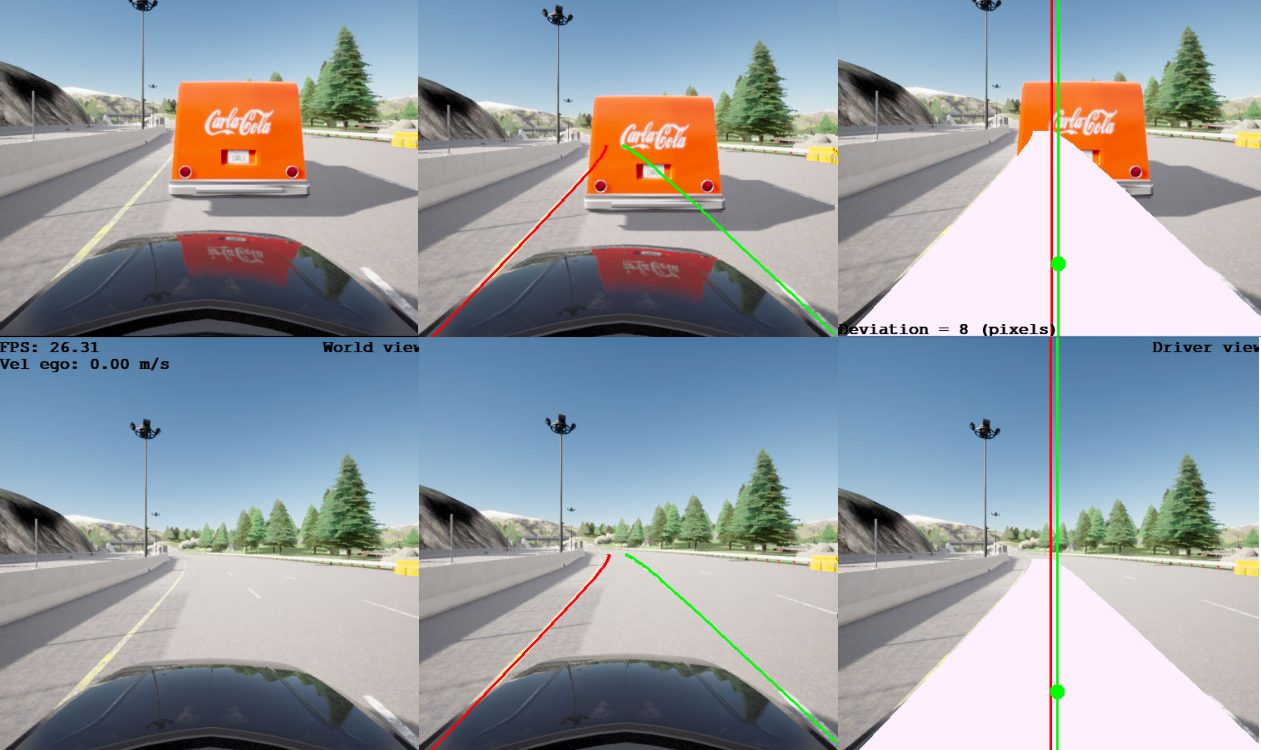
\includegraphics[width=13cm]{figs/Diseño/lane/ground_truth.png}
\caption{Detección de carril basada en \textit{ground thruth}.}
\label{fig:gt_final_carril}
\end{figure}

\newpage

Al basarse en información obtenida directamente del simulador CARLA, este enfoque resulta más fiable que la detección de carril mediante \ac{DL}, puesto que, a pesar de los posibles obstáculos que puedan afectar la visibilidad, es capaz de seguir detectando el carril como se muestra en la Figura \ref{fig:gt_final_carril}. Dado que este \ac{TFG} se centra en la generación de comportamientos para la toma de decisiones, es fundamental contar con una percepción lo más precisa posible durante los entrenamientos para evitar que influya negativamente en el aprendizaje del modelo. Por ello, esta será la técnica empleada en el proceso de entrenamiento. Además, en ciertos escenarios se da la presencia de un vehículo delantero que puede ocultar temporalmente las líneas del carril, lo que hace aún más necesario un método de detección robusto y fiable en cualquier tipo de situación.

\subsection{Segmentación de la calzada}
\label{sec:per_ef}

Comprender la ubicación del carril por el que circulamos es fundamental, pero también buscamos obtener más información sobre la calzada: sus límites, su área y la presencia de otros carriles. Para ello, incluimos en el sistema de percepción la red neuronal de segmentación semántica EfficientVit, descrita en la sección \ref{sec:ef}. Al igual que para el carril, necesitamos una representación simplificada de la misma. Para ello, analizamos la máscara de segmentación que nos proporciona EfficientVit calculando su área, centro de masas y \textit{n} puntos igualmente espaciados en el eje \textit{y} de cada límite lateral de la calzada. Con el fin proporcionar información más valiosa al modelo, seleccionamos solo un cuarto de los puntos de la parte totalmente vertical, como se puede apreciar en la Figura \ref{fig:seg_params}. Esta funcionalidad ha sido implementada principalmente con la librería NumPy para maximizar la eficiencia computacional.
\begin{figure}[ht]
\centering
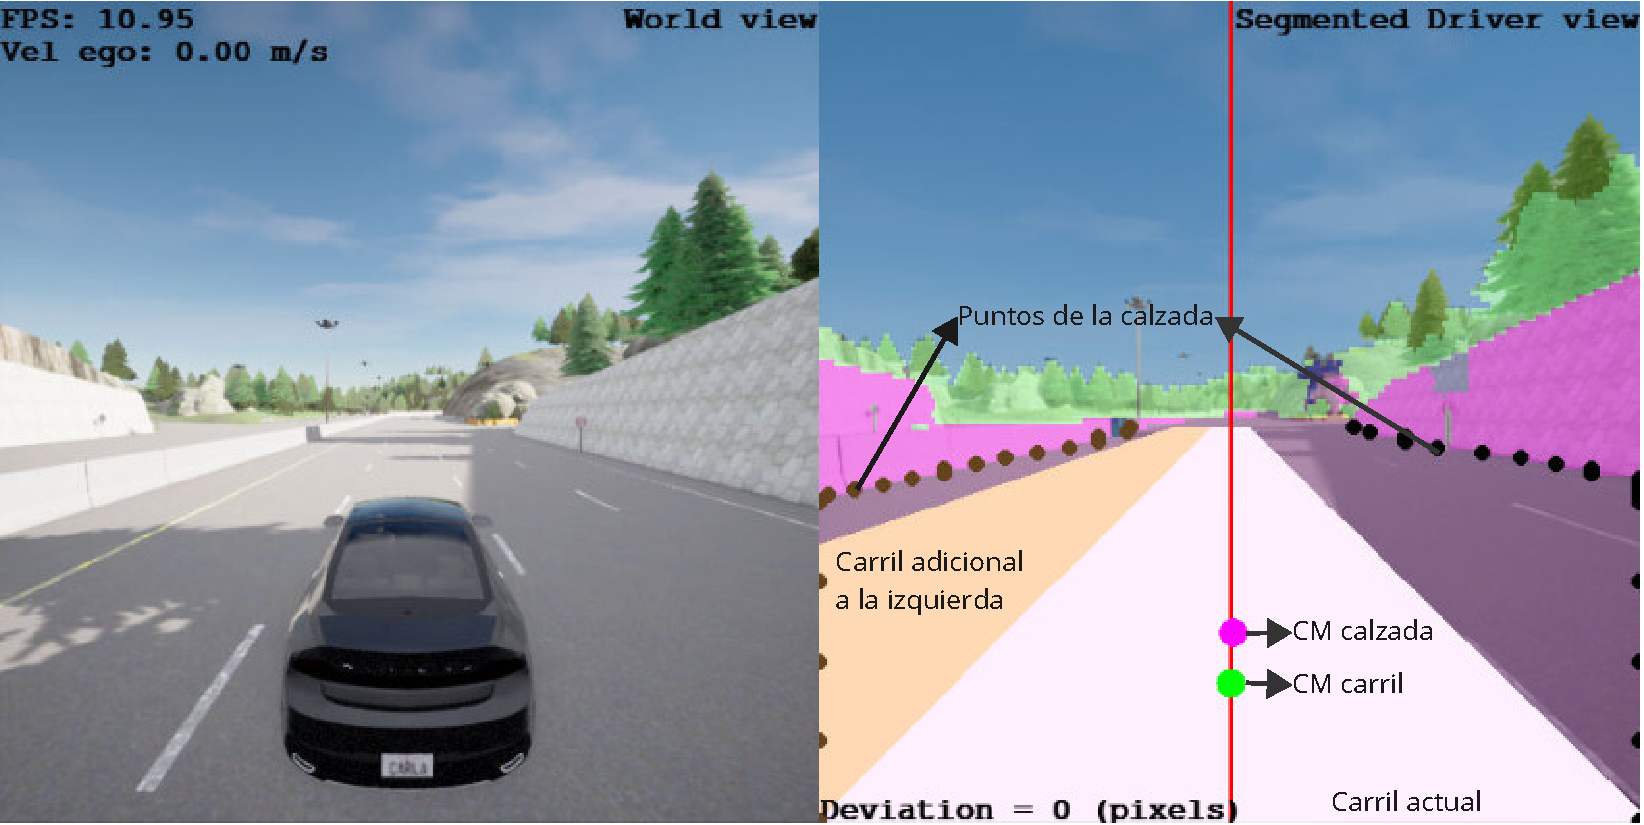
\includegraphics[width=13cm]{figs/Diseño/seg_points.pdf}
\caption{Representación de la calzada: carriles, superficie, centro de masas y límites.}
\label{fig:seg_params}
\end{figure}

También se utiliza la segmentación para comprobar el porcentaje del área del carril que es calzada y para saber si hay un carril a la izquierda. Esto nos proporciona más conocimiento acerca del entorno, lo que nos permitiría realizar maniobras como un adelantamiento, donde es necesario verificar la existencia de un carril al que podamos desplazarnos. Para hacer esta última comprobación, replicamos el carril actual a la izquierda y comprobamos que porcentaje de ese área es calzada, zona naranja en la Figura \ref{fig:seg_params}.

\section{Percepción basada en LiDAR}

La percepción visual nos aporta mucha información sobre la calzada, pero también necesitamos detectar otros elementos que pueda haber en la carretera. Para ello, añadimos un nuevo sensor a la percepción, el \ac{LiDAR}. Si bien es posible detectar otros vehículos mediante la cámara y estimar su distancia, el \ac{LiDAR} ofrece mediciones más fiables, especialmente en condiciones adversas como lluvia o baja iluminación. Por lo tanto, para garantizar la seguridad en la conducción autónoma, optamos por utilizar el \ac{LiDAR} para la detección de otros vehículos en la vía.

El \ac{LiDAR} es un sensor simulado de CARLA que proporciona como salida una nube de puntos que indica la distancia y la posición de los objetos en el entorno, permitiendo una reconstrucción de la escena para la percepción y navegación del vehículo autónomo. Se configura el \ac{LiDAR} con un alcance máximo de 20 metros, distancia suficiente para detectar obstáculos en la carretera, en nuestro caso otros vehículos. Para la representación gráfica de la información del \ac{LiDAR}, mostramos cada uno de los puntos de la nube en 2D, coordenadas \textit{x} e \textit{y}. Con el fin de mejorar la visualización, se ha interpolado el color de cada punto según su intensidad, siendo tonos rojos los valores más altos y azules los más bajos, y el tamaño según su altura, a mayor elevación mayor tamaño.

\begin{figure}[ht]
\centering
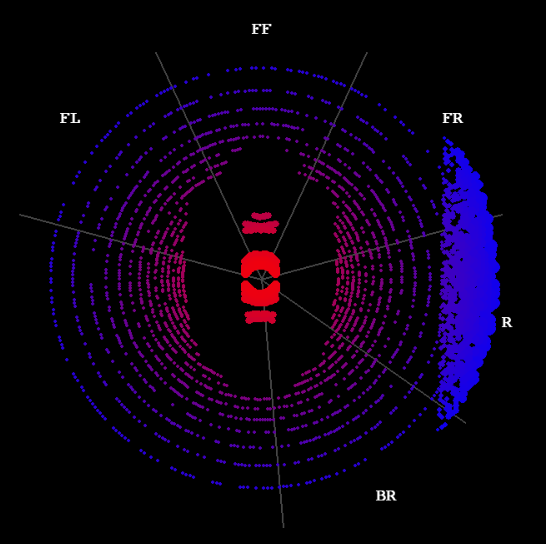
\includegraphics[width=7cm]{figs/Diseño/lidar/interpolate.png}
\caption{Visualización de la nube de puntos y zonas del \ac{LiDAR}.}
\label{fig:interpolate_lidar}
\end{figure}

Para identificar otros vehículos en la trayectoria del coche, nos enfocamos en analizar la zona frontal del \ac{LiDAR}, con una amplitud de 150º, dividida en tres subzonas de 50º: \textit{front-left}, \textit{front}, \textit{front-right}, como se ve en la Figura \ref{fig:interpolate_lidar}. Para determinar los ángulos que delimitan estas zonas, independientemente de cómo se disponga el \ac{LiDAR} en el vehículo, debemos tener en cuenta su rotación en el eje z (\textit{yaw}). Partiendo del \textit{yaw} del \ac{LiDAR}, si queremos calcular los ángulos límite debemos sumarle y restarle la mitad del ángulo frontal. Posteriormente, este ángulo se acota en un rango de [-180º, 180º]. Aunque ya hemos encontrado los ángulos extremos, es necesario calcular los dos ángulos intermedios que delimitan las tres subzonas. Para ello, sumamos la amplitud de cada subzona al primer ángulo límite y se la restamos al segundo. Posteriormente, se incluyó la posibilidad de añadir dos nuevas subzonas en la parte lateral derecha del \ac{LiDAR}, \textit{right} y \textit{back-right}, permitiendo así la detección de obstáculos en un rango más amplio. En nuestro caso, con un \textit{yaw} de 90º, obtenemos los ángulos: [-165.0, -115.0, -65.0, -15.0, 35.0, 85.0].

\begin{code}[h]
\begin{lstlisting}[language=Python]
angle1 = get_angle_range(-self._front_angle / 2 - yaw)
angle2 = get_angle_range(self._front_angle / 2 - yaw)

angle1_add = get_angle_range(angle1 + self._front_angle / 3)
angle2_sub = get_angle_range(angle2 - self._front_angle / 3)        
self._angles = [angle1, angle1_add, angle2_sub, angle2]

if self._back:
	self._angles.append(angle2 + self._front_angle / 3)
	self._angles.append(angle2 + (self._front_angle / 3) * 2)
\end{lstlisting}
\caption[Cálculo de los ángulos de la zona del \ac{LiDAR}]{Cálculo de los ángulos del \ac{LiDAR}.}
\label{cod:angle_lidar}
\end{code}

\newpage

Como se puede observar en el dibujo \ref{fig:dib_angle}, dependiendo de que ángulo sea mayor, debemos seguir un criterio u otro para determinar si un punto pertenece o no a la zona de interés o a una subzona concreta.
\begin{figure}[ht]
  \centering
  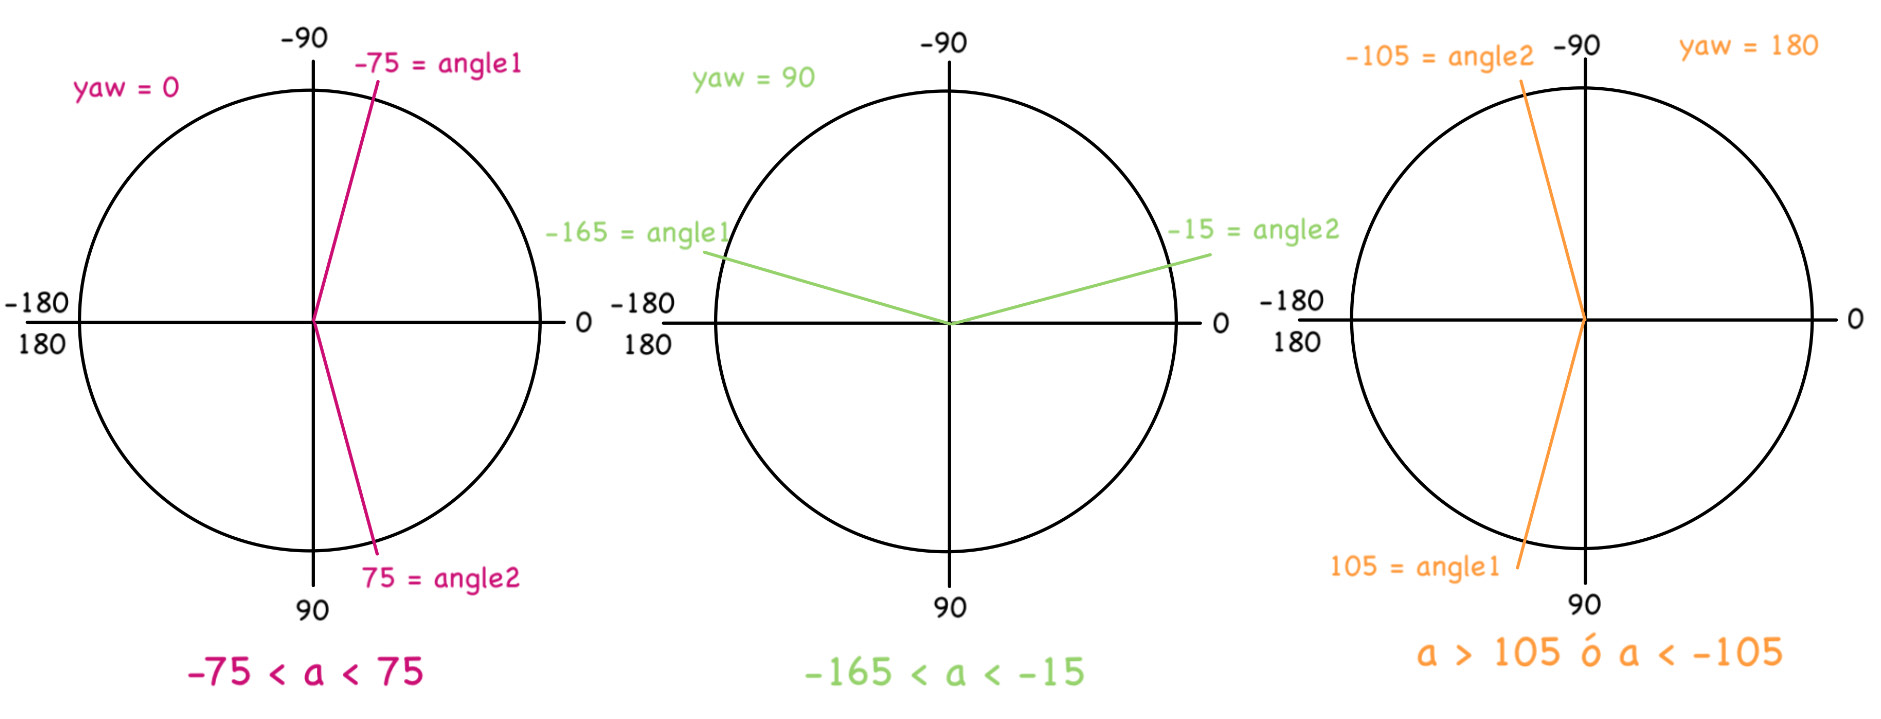
\includegraphics[width=10cm]{figs/Diseño/lidar/draw_angles.jpg}
  \caption{Criterio para saber a qué zona pertenece un punto del \ac{LiDAR}.}
  \label{fig:dib_angle}
\end{figure}

Para tener información adicional, se ha creado un cálculo de estadísticas para cada subzona: mínimo, media, mediana y desviación estándar. Dado que el \ac{LiDAR} se ha ubicado en el techo del vehículo y no en la parte frontal, algunos elementos detectados corresponden al propio coche (puntos rojos), como se observa en la Figura \ref{fig:stats_lidar}. Para evitar que afecten los cálculos estadísticos, se ha aplicado un filtrado por intensidad para eliminarlos. De la misma manera, filtramos por altura para eliminar todos los puntos correspondientes a la calzada y otros elementos del entorno externos a la carretera (montañas, árboles…), quedándonos solo con información relevante para la conducción.
\begin{figure}[ht]
  \centering
  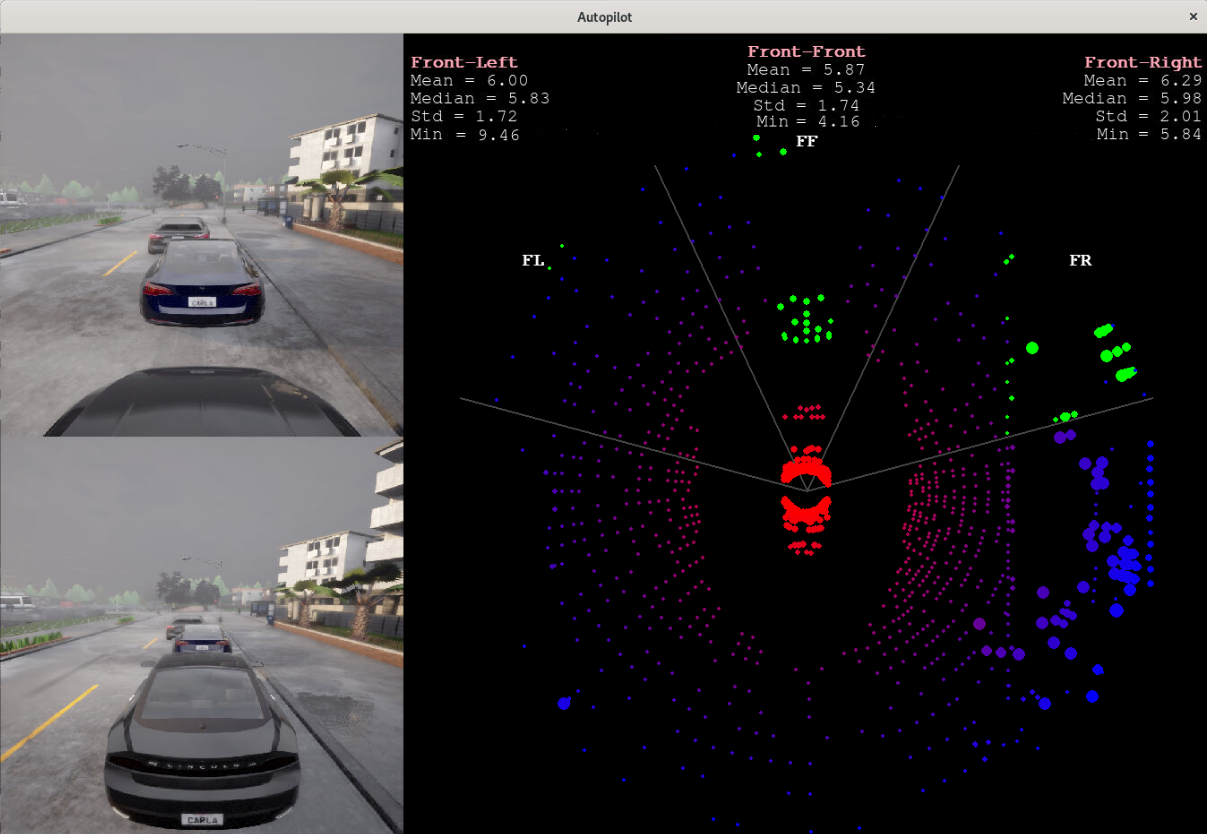
\includegraphics[width=11cm]{figs/Diseño/lidar/stats.png}
  \caption{Filtrado de puntos y cálculo de estadísticas del \ac{LiDAR}.}
  \label{fig:stats_lidar}
\end{figure}

\newpage

Se ha implementado una función que extrae un número determinado de puntos de cada subzona, los cuales están ordenados y distribuidos de manera equidistante a lo largo del eje \textit{x}. Estos puntos se utilizan como observaciones para los modelos, garantizando una representación precisa y bien estructurada de la información obtenida del \ac{LiDAR}. En la Figura \ref{fig:laser_front}, se muestra este proceso en la subzona frontal del \ac{LiDAR}, colocando un vehículo delante a diferentes distancias.
\begin{figure}[ht]
\centering
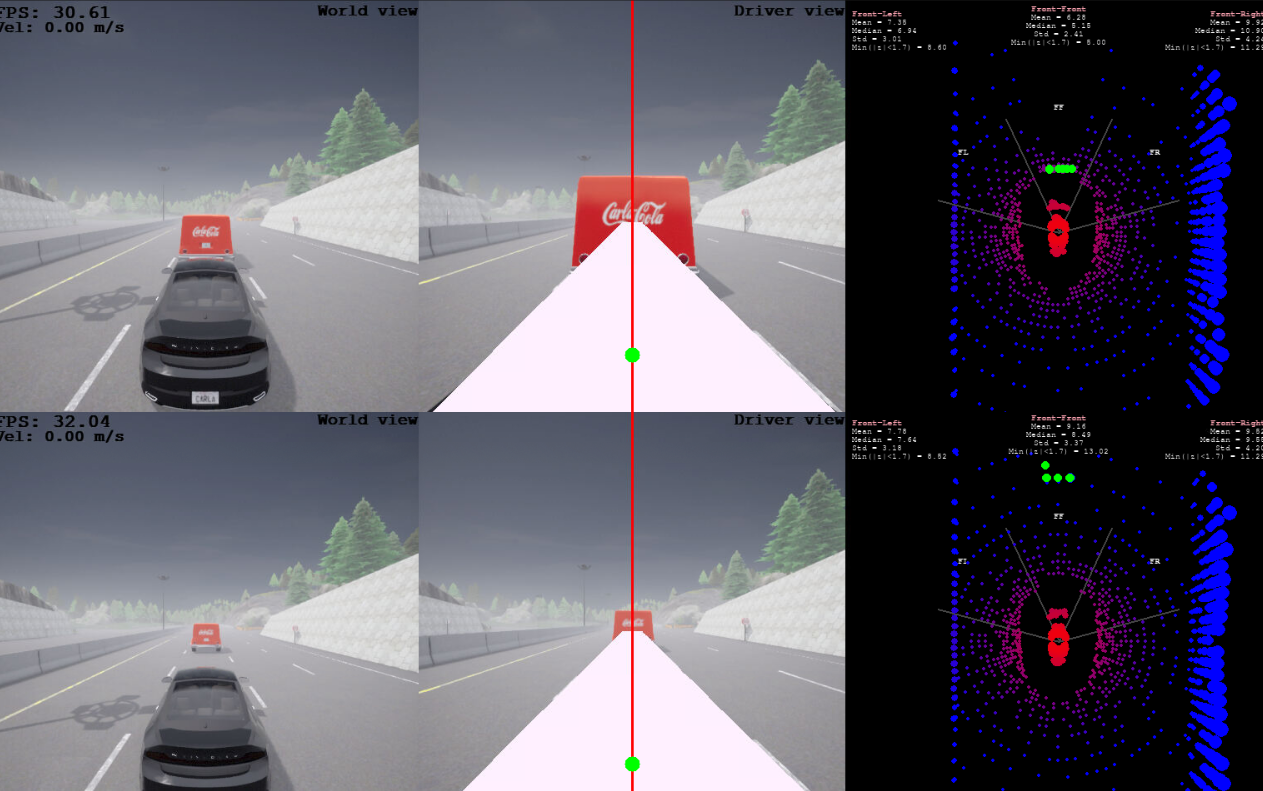
\includegraphics[width=12cm]{figs/Diseño/lidar/laser_front.png}
\caption{Selección de puntos de la subzona frontal del \ac{LiDAR}.}
\label{fig:laser_front}
\end{figure}

Se realizó un \textit{profiling} para evaluar las latencias y detectar los procesos con mayor consumo de tiempo en el código, con el objetivo de optimizar su eficiencia. Como se observa en la Figura \ref{fig:profiling}, la mayor parte del tiempo de cómputo se destina a la predicción con EfficientVit, mientras que el resto de los procesos presentan latencias acordes a su carga computacional y no suponen un inconveniente significativo.
\begin{figure}[ht]
  \centering
  \includegraphics[width=\textwidth]{figs/Diseño/profiling.png}
  \caption{\textit{Profiling} del proceso de percepción.}
  \label{fig:profiling}
\end{figure}

Tras analizar los resultados desde un enfoque tanto computacional como de desempeño, se ha concluido que la combinación de EfficientVit para la segmentación de la calzada, \textit{ground truth} para detección del carril y el \ac{LiDAR} como fuente adicional de datos para detectar obstáculos en la carretera, permite un equilibrio entre precisión y eficiencia de procesamiento, al menos para una primera parte de entrenamiento en simulación. Dado que la latencia total del sistema es de aproximadamente 70 ms por iteración, esto implica que el sistema puede actualizarse a una tasa de 14 \ac{FPS} en el servidor Thor, descrito en la sección \ref{sec:thor}. Sin embargo, en un entorno real no tenemos esa percepción perfecta basada en \textit{ground truth}, ya que es una técnica exclusiva del simulador CARLA. Si adoptamos por un enfoque más realista, utilizando la detección de carril basada en \ac{DL}, obtenemos latencias de 75 ms, lo cual no supone una diferencia significativa en términos de coste computacional. Este rendimiento es adecuado para aplicaciones en tiempo real, permitiendo así lograr comportamientos reactivos y robustos en entornos dinámicos.

\section{Toma de decisiones}

El módulo de toma de decisiones permite a nuestro sistema interpretar el entorno de manera eficiente según los datos procedentes de la percepción. Este sistema de conducción autónoma debe ser capaz de seguir el carril con precisión, mantener un control de crucero adaptativo respetando la distancia de seguridad respecto al vehículo delantero y realizar maniobras de adelantamiento completa de forma segura. Debe tener la capacidad de tomar decisiones informadas, seguras y óptimas, garantizando comportamientos realistas y eficientes. Para ello, se han implementado dos tipos de soluciones: una basada en técnicas tradicionales de conducción autónoma y otra en \ac{ML}, que permite gestionar la información de manera más eficiente al adaptarse mejor a las condiciones cambiantes del entorno, a diferencia de las soluciones tradicionales que se rigen por normas predefinidas.

Para los entrenamientos y ajustes de los modelos de conducción autónoma, primero debemos elegir uno o varios circuitos para nuestro modelo. Para ello, hemos elegido el Town04 de CARLA, ya que incluye tramos largos y sin intersecciones. En una primera aproximación de este \ac{TFG}, no se abordó la gestión de intersecciones debido a la complejidad adicional que implican. Como se muestra en la Figura \ref{fig:mapa}, se han definido cuatro rutas. Las rutas uno, dos y tres, representadas en rosa, amarillo y verde, respectivamente, se utilizan para el entrenamiento, mientras que la ruta cuatro, en color azul, se reserva para evaluar el modelo en inferencia y comprobar su capacidad de generalización. Cada una de estas rutas comienza siempre en el mismo punto (círculo junto al número), pero difieren en el tramo del mapa y la dirección de inicio: curva a la derecha, línea recta y curva a la izquierda, con el objetivo de evitar \textit{overfitting} en el modelo. También se incluyó un nuevo circuito en el Town03 de CARLA para realizar pruebas en inferencia y evaluar la capacidad de adaptación del modelo a un entorno distinto al del entrenamiento, como se observa en la Figura \ref{fig:cir3}.

\begin{figure}[ht]
\centering
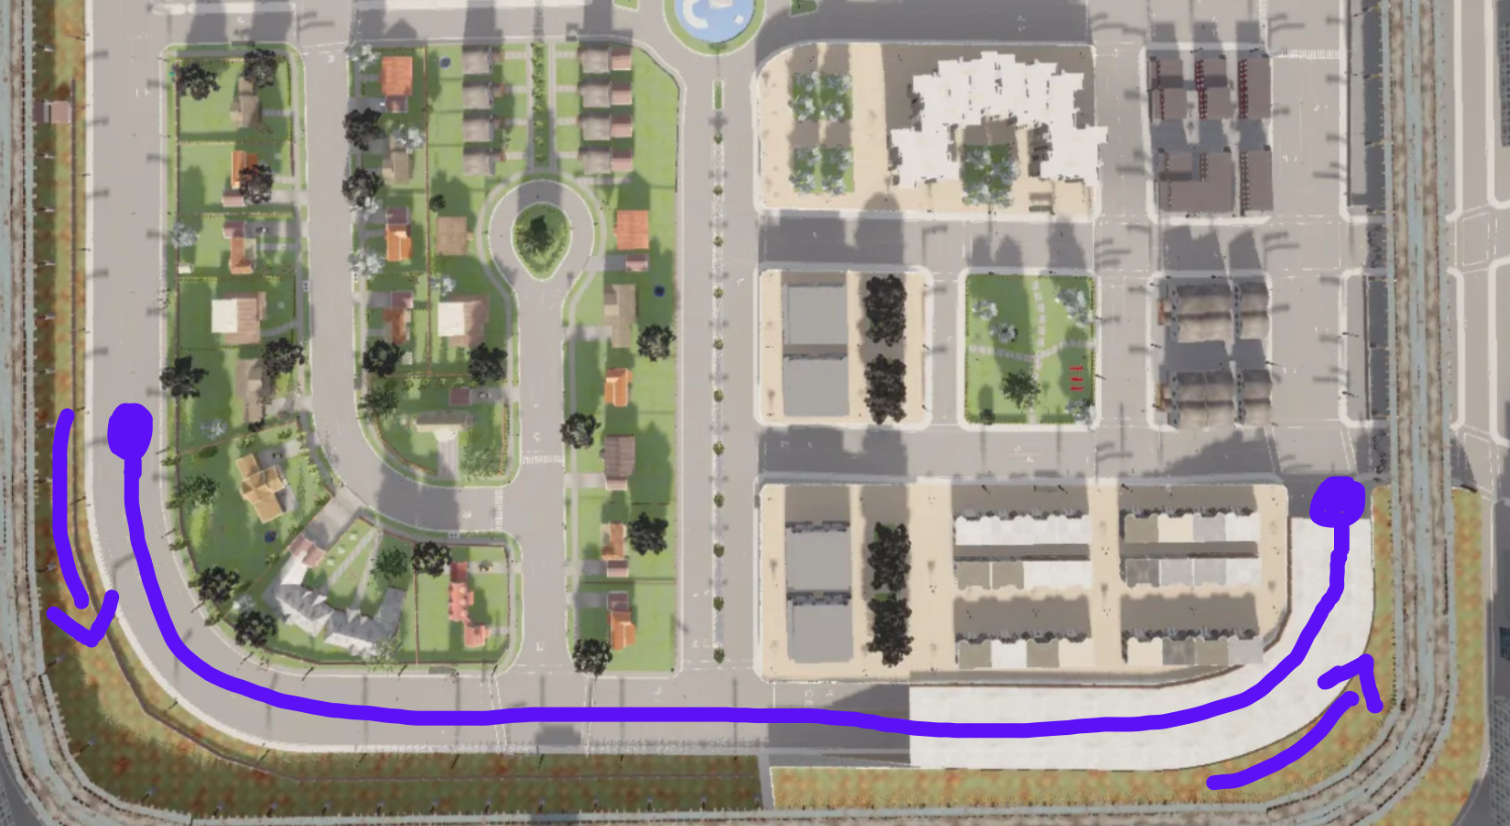
\includegraphics[width=7cm]{figs/Diseño/cir3.jpg}
\caption{Mapa de un circuito no visto durante el entrenamiento (Town03).}
\label{fig:cir3}
\end{figure}

\begin{figure}[ht]
  \centering
  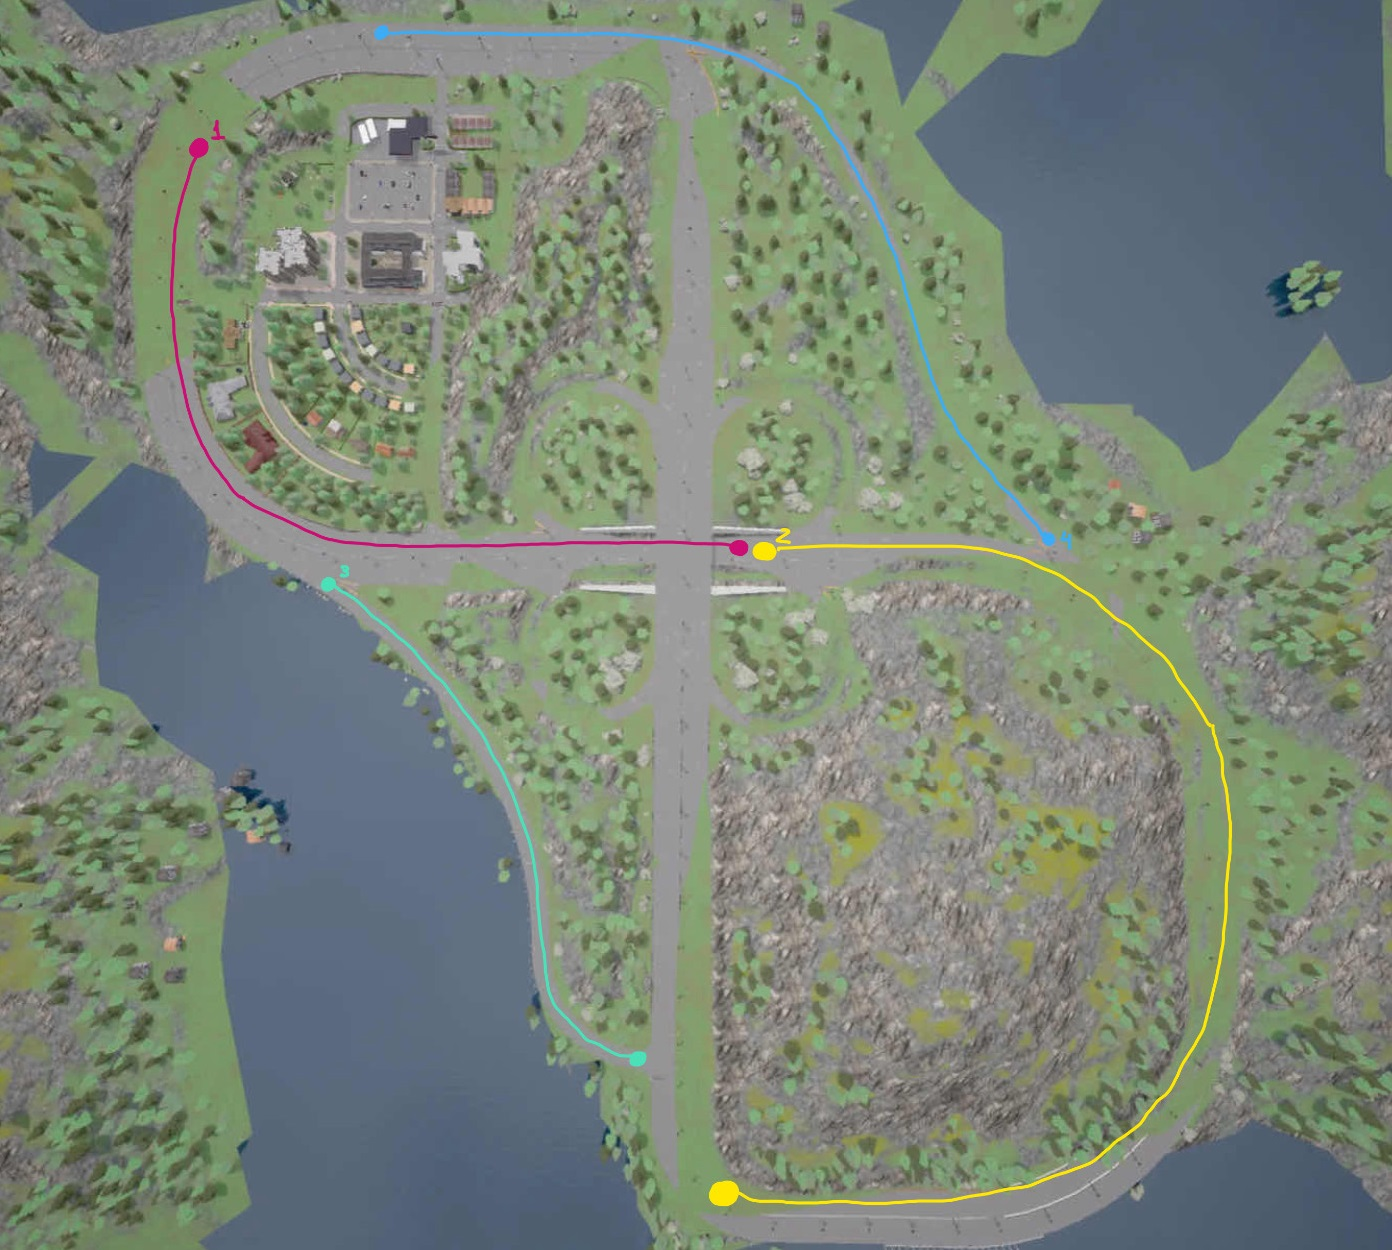
\includegraphics[width=10cm]{figs/Diseño/mapa.jpeg}
  \caption{Mapa de los circuitos de entrenamiento en CARLA (Town04).}
  \label{fig:mapa}
\end{figure}

\newpage

\subsection{Sigue carril basado en un controlador PID}

Existen técnicas de control clásico que funcionan eficientemente para ciertas habilidades de conducción donde los escenarios no son cambiantes ni dinámicos, pero es muy difícil su convergencia a comportamientos realistas cuando el entorno es complejo. Un controlador \ac{PID} es un tipo de control tradicional ampliamente utilizado en sistemas automáticos para ajustar una variable y mantenerla en un valor deseado. En conducción autónoma, se usa para mantener un vehículo en el carril ajustando el ángulo del volante según la desviación respecto al centro del carril.

Para el seguimiento de carril basado en un controlador tradicional, se ha implementado un controlador PD para ajustar el giro y un controlador P para regular el acelerador, con el objetivo de mantener una velocidad constante de 10 m/s y seguir el carril de forma precisa. A continuación, se presentan las constantes definidas para los controladores:
\begin{code}[h]
\begin{lstlisting}[language=Python]
self._kp_dev = 1 / (SIZE_CAMERA / 2)
self._kd_dev = -self._kp_dev / 1.7
self._kp_vel = 1.75
\end{lstlisting}
\caption[Definición de constantes para el controlador \ac{PID}]{Definición de constantes para el controlador \ac{PID}.}
\label{cod:const_pid}
\end{code}

Para controlar el acelerador, primero calculamos la diferencia entre la velocidad actual del coche y la velocidad objetivo. Este valor se normaliza y se introduce en el controlador proporcional. El valor del acelerador se limita al rango [0.0, 0.5]. Por otro lado, en el módulo de percepción, ya habíamos calculado la desviación respecto al centro del carril del vehículo. Esta desviación representa el error que recibe  el controlador PD. El componente proporcional se encarga de normalizar el error en el rango de giro [0.0, 1.0], mientras que el signo del error ya indica el sentido del giro. Si el error supera cierto umbral, lo incrementamos ligeramente para mejorar el rendimiento en las curvas. El componente derivativo evita movimientos oscilatorios al salir de las curvas, ya que tiene en cuenta el error anterior atenuado. Este componente resta el valor del error anterior, pero solo se considera si su signo es diferente al del error actual, ya que, de lo contrario, podría causar inestabilidad y afectar negativamente la conducción durante las curvas.

\begin{code}[h]
\begin{lstlisting}[language=Python]
# Different sign
if (self._error > 0 and self._prev_error < 0) or (self._error < 0 and self._prev_error > 0):
    self._prev_error = 0       

# Increase in error
if error > 20:
    error *= 1.15

control.steer = self._kp * error + self._kd * self._prev_error
\end{lstlisting}
\caption[Regulación del giro mediante el controlador \ac{PID}]{Regulación del giro mediante el controlador \ac{PID}.}
\label{cod:pid_giro}
\end{code}

En los histogramas \ref{fig:comparativa_pid}(a) se muestra la velocidad en m/s del coche autónomo y el error respecto al centro del carril en píxeles durante el circuito en el que se ajustó\footnote{\url{https://youtu.be/Me3KQ3X_n-0}} el controlador \ac{PID} (circuito 3 de la Figura \ref{fig:mapa}), mientras que en los histogramas \ref{fig:comparativa_pid}(b) se presenta la misma información, pero en un circuito en el que no se realizó el ajuste\footnote{\url{https://youtu.be/ygVov8ERqFI}} (circuito de la Figura \ref{fig:cir3}). Los datos se recopilaron durante 30 segundos en ambos casos. En los dos circuitos, podemos ver que el coche acelera al inicio, alcanzando rápidamente una velocidad de 10 m/s, la cual se mantiene constante durante todo el recorrido. Sin embargo, se observan diferencias significativas en la precisión del seguimiento de carril. Mientras que en el circuito ajustado el histograma de la desviación está centrado, en el circuito sin ajuste la distribución se dispersa notablemente, alcanzando valores entre 35 y 45 píxeles con una frecuencia considerable. A pesar de que el circuito dispone de curvas pronunciadas, estas desviaciones no deberían ser tan altas, puesto que el vehículo debería mantenerse dentro de los límites del carril en todo momento para garantizar una conducción segura y eficiente. Esto evidencia que un controlador \ac{PID} no es capaz de generalizar adecuadamente ante entornos cambiantes, provocando inestabilidad en la trayectoria y el comportamiento del vehículo, lo cual no es óptimo en entornos de conducción autónoma.

\begin{figure}[ht]
\centering
\subfigure[Histogramas del circuito ajustado (Town04).]{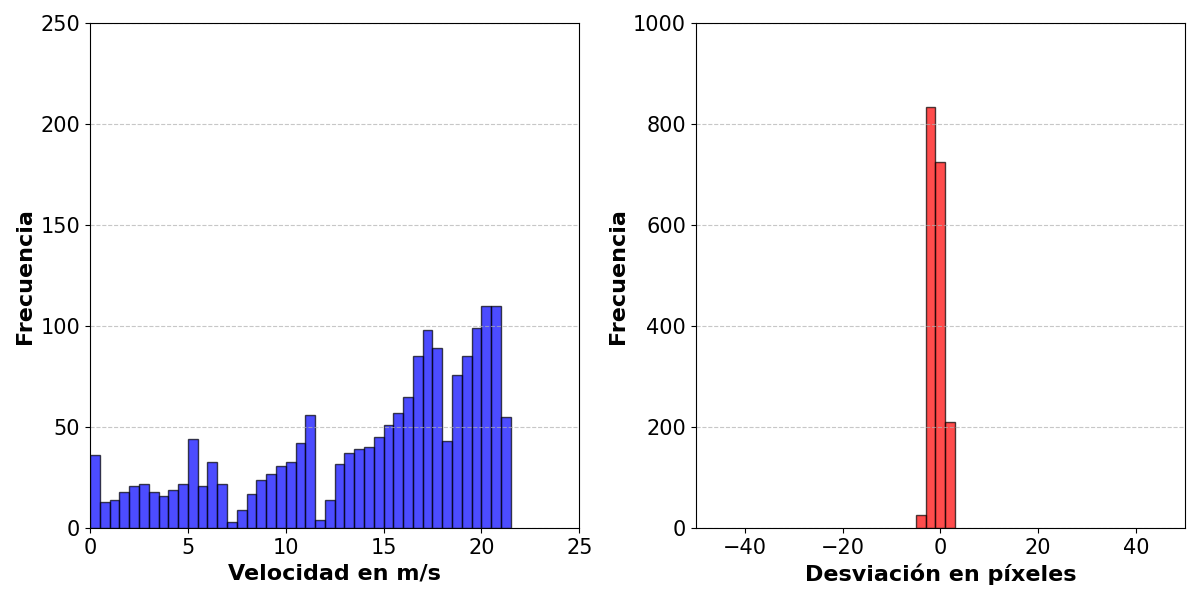
\includegraphics[width=0.45\textwidth]{figs/Diseño/pid/ajustado.png} \label{fig:pid_ajus}}
\hfill
\subfigure[Histogramas del circuito no ajustado (Town03).]{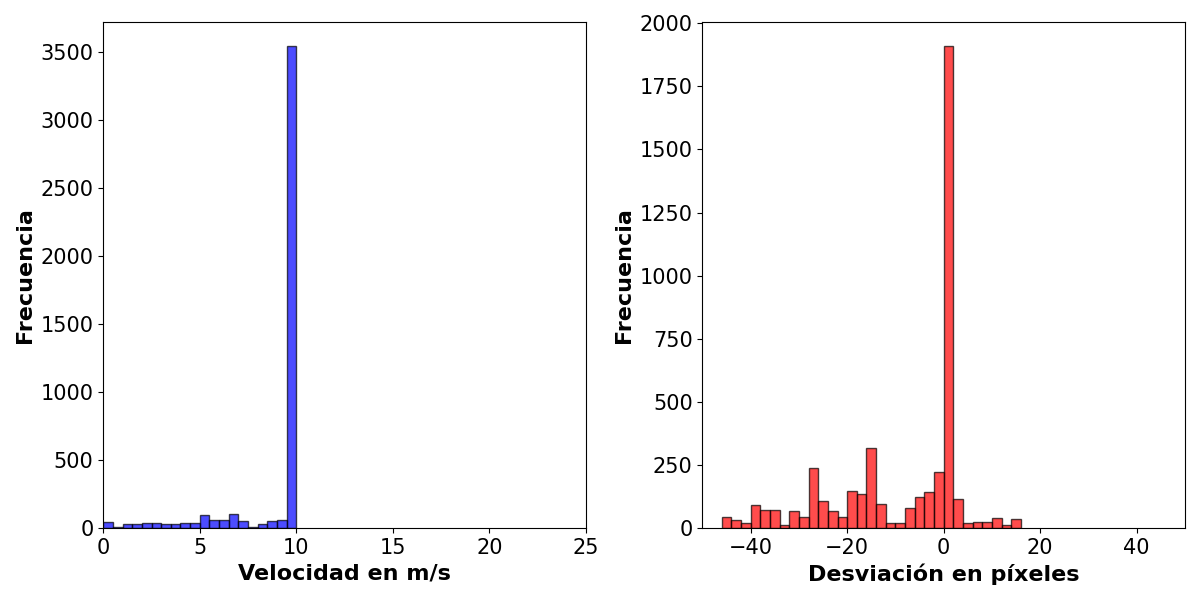
\includegraphics[width=0.45\textwidth]{figs/Diseño/pid/no_ajustado.png} \label{fig:pid_no_ajus}}
\caption{Comparativa de la velocidad y desviación del vehículo basado en un controlador \ac{PID}.}
\label{fig:comparativa_pid}
\end{figure}

El controlador \ac{PID} es una solución sencilla para corregir el error de la desviación con el objetivo de seguir un carril y, por lo tanto, tiene un bajo costo computacional de apenas 20 µs. La latencia total depende principalmente del tiempo empleado en la detección del carril, aproximadamente 10-11 ms. Nuestro sistema puede operar a una tasa de 90-100 \ac{FPS}, haciéndolo adecuado para aplicaciones en tiempo real donde se requiere un comportamiento reactivo.

\subsection{Seguimiento de carril basado en DQN}

Como se describió en la sección \ref{sec:stable_baselines3}, \ac{DQN} es un algoritmo \textit{off policy} que permite un espacio de observaciones continuo, pero el espacio de acciones es discreto. Ahora que ya sabemos cómo funciona el algoritmo \ac{DQN}, es el momento de construir el entorno de entrenamiento para que nuestro coche autónomo sea capaz de seguir el carril. Los circuitos de entrenamiento del modelo ya fueron definidos previamente en la Figura \ref{fig:mapa}, procurando que fuesen variados para prevenir el \textit{overfitting}. Por otro lado, el espacio de observaciones coincide con el espacio de estados y está basado en un diccionario, lo que nos lleva a emplear la política \textit{MultiInputPolicy}, descrita también en la sección \ref{sec:stable_baselines3}. Las observaciones se normalizan para facilitar el aprendizaje al modelo e incluyen la siguiente información:
\begin{itemize}
		\item Desviación del carril.
		\item Área del carril.
		\item Cinco puntos de la línea izquierda del carril.
		\item Cinco puntos de la línea derecha del carril.
		\item Centro de masas del carril.
\end{itemize}

\begin{figure}[ht]
  \centering
  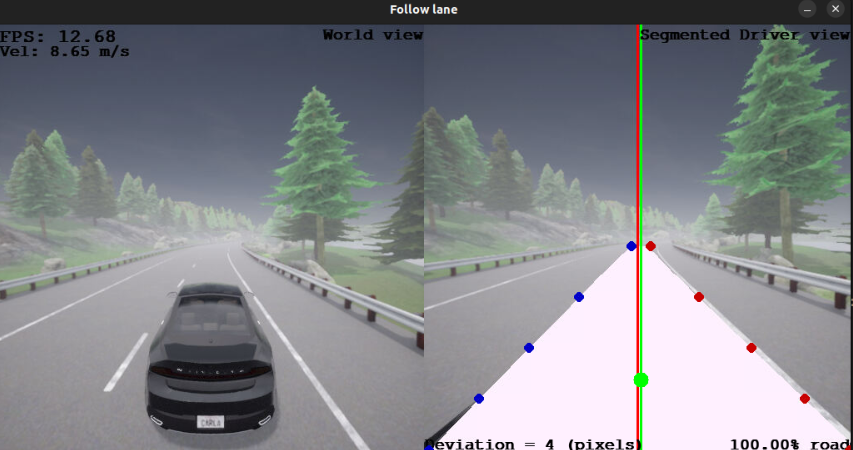
\includegraphics[width=8cm]{figs/Diseño/discrete/obs_dqn.png}
  \caption{Observaciones seguimiento de carril basado en \ac{DQN}.}
  \label{fig:dqn_obs}
\end{figure}

Como se mencionó al inicio, \ac{DQN} permite un espacio de acciones discreto. Las acciones están compuestas por un comando de acelerador y otro de giro. Para combinarlos, hemos seguido la regla de que, a mayor aceleración, menor es el giro. En total, se han definido 21 acciones entre las cuales el agente podrá seleccionar aquellas que maximicen la recompensa en cada situación.
\begin{code}[h]
\begin{lstlisting}[language=Python]

self.action_to_control = {
    0: (0.5, 0.0),
    1: (0.45, 0.01), 
    2: (0.45, -0.01),
    3: (0.4, 0.02),
    4: (0.4, -0.02),
    5: (0.4, 0.04),
    6: (0.4, -0.04),
    7: (0.4, 0.06),
    8: (0.4, -0.06),
    9: (0.4, 0.08),
    10: (0.4, -0.08),
    11: (0.3, 0.1),
    12: (0.3, -0.1),
    13: (0.3, 0.12),
    14: (0.3, -0.12),
    15: (0.2, 0.14),
    16: (0.2, -0.14),
    17: (0.2, 0.16),
    18: (0.2, -0.16),
    19: (0.1, 0.18),
    20: (0.1, -0.18)
}
\end{lstlisting}
\caption[Acciones disponibles para el seguimiento de carril basado en \ac{DQN}]{Acciones disponibles para el seguimiento de carril basado en \ac{DQN}.}
\label{cod:acc_dqn}
\end{code}

\newpage

Nuestro objetivo es que el coche circule por el centro del carril sin desviarse, manteniendo una conducción fluida y a velocidades óptimas. Para lograrlo, hemos diseñado una función de recompensa que se basa principalmente en la desviación del carril y en la velocidad actual del coche, normalizando y ponderando estos valores según sus pesos. Sin embargo, si el coche colisiona contra un elemento del entorno (detectado con sensor de colisión, descrito en la sección \ref{sec:carla}) y pierde o cambia de carril, el episodio se detiene y se asigna una recompensa negativa.
  \begin{myequation}[h]
    \begin{equation} 
      \text{reward} = 0.8 \cdot r_{\text{dev}} + 0.2 \cdot r_{\text{vel}} 
    \end{equation} 
    \caption{Función de recompensa para el sigue-carril basado en \ac{DQN}.}
\label{eq:rew_ppo}
  \end{myequation}
\begin{code}[h]
\begin{lstlisting}[language=Python]
if error == None:
      r_dev = (MAX_DEV - abs(np.clip(self._dev, -MAX_DEV, MAX_DEV))) / MAX_DEV
      r_vel = np.clip(self._velocity, 0.0, self._max_vel) / self._max_vel
      reward = 0.8 * r_dev + 0.2 * r_vel
else:
      reward = -30
\end{lstlisting}
\caption[Función de recompensa sigue-carril basado en \ac{DQN}]{Función de recompensa sigue-carril basado en \ac{DQN}.}
\label{cod:rew_dqn}
\end{code}

\newpage

Durante los entrenamientos utilizamos el modo síncrono de CARLA, en el cual el cliente puede indicar al servidor cuándo ejecutar con la función  \textit{world.tick()} y el tiempo simulado de cada \textit{steps} con el parámetro \textit{fixed\_delta\_seconds}, tras el cual la simulación se detiene hasta que se llama de nuevo a \textit{tick}. Hemos utilizado un \textit{fixed\_delta\_seconds} de 50 ms en CARLA, lo que equivale a entrenar a 20 \ac{FPS}, por lo tanto, en inferencia necesitamos operar al menos a esta velocidad. Los entrenamientos tuvieron una duración de 26 horas en el servidor Thor. Para lograr una exploración eficiente y alcanzar una solución óptima, fue necesario un alto número de \textit{steps}, llegando hasta ocho millones. El tamaño de la memoria es de un millón de experiencias, por lo que la memoria se actualiza completamente un total de ocho veces. Tras realizar diversas pruebas, identificamos los hiperparámetros de entrenamiento que proporcionan los mejores resultados.
\begin{table}[ht]
\centering
\renewcommand{\arraystretch}{1.2} % Aumenta el espacio entre filas para mejor legibilidad
\begin{tabular}{|l|l|p{9cm}|} % Ajusta el ancho de la última columna
\hline
\textbf{Hiperparámetro} & \textbf{Valor} & \textbf{Descripción} \\ \hline
buffer\_size & 1,000,000 & Tamaño de la memoria (\textit{replay memory}) \\ \hline
train\_freq & 256 & Frecuencia de entrenamiento: cada cuántos pasos se actualiza la red neuronal \\ \hline
exploration\_fraction & 0.8 & Fracción de exploración \\ \hline
exploration\_final\_eps & 0.0 & Valor final del parámetro de exploración \\ \hline
n\_timesteps & 8,000,000 & Número total de \textit{steps} para el entrenamiento \\ \hline
\end{tabular}
\caption{Hiperparámetros de entrenamiento para el sigue-carril basado en \ac{DQN}.}
\label{tab:hiperparametros}
\end{table}

La frecuencia de entrenamiento resultó ser un factor clave en el proceso, al principio se utilizó un valor menor, pero los modelos no lograban converger. Esto se debe a que, al actualizar el modelo con ejemplares demasiado consecutivos, los datos están altamente correlacionados, generando inestabilidad y dificultando la convergencia. Sin embargo, al aumentar el valor de este hiperparámetro, la memoria acumula datos más diversos y significativos antes de actualizar los pesos del modelo.

En la gráfica \ref{fig:train_dqn}, se puede observar cómo el modelo finalmente converge. El primer \textit{plot} muestra la recompensa obtenida en cada episodio (azul) y la recompensa promedio acumulada por episodio (amarillo), que finalmente se estabiliza en un valor de 3.500 aproximadamente. En el segundo \textit{plot}, se muestra el número de \textit{steps} por episodio. A pesar de que al inicio los episodios son más largos y, por lo tanto, acumulan una mayor recompensa, no es ese el comportamiento que deseamos. Buscamos que el modelo alcance velocidades significativas, por lo que, a medida que aprende, los episodios tienen menos \textit{steps}, logrando completar el circuito más rápido sin comprometer la eficiencia. Los puntos verdes indican que el agente ha sido capaz de completar con éxito el circuito, mientras que los rojos señalan que ha tomado una acción que ha provocado el fin del episodio, como salirse del carril. Finalmente, en el último \textit{plot}, se muestra cómo evoluciona el ratio de exploración, su valor se reduce gradualmente durante el 80\% del entrenamiento y, a partir de ese punto, se dejan de realizar acciones aleatorias.
\begin{figure}[ht]
\centering
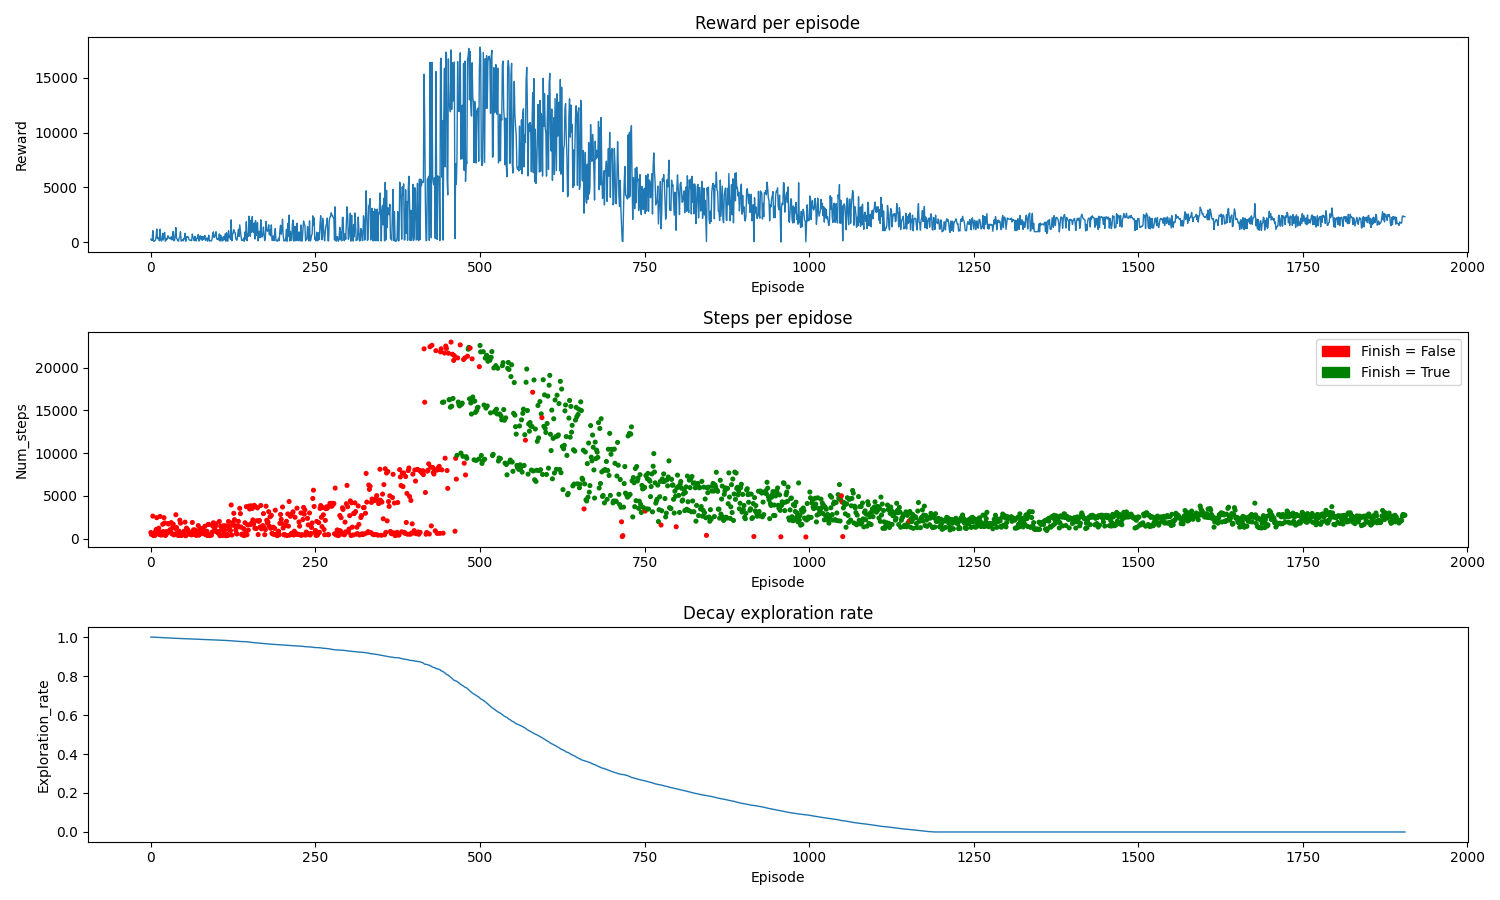
\includegraphics[width=\textwidth]{figs/Diseño/discrete/train_dqn.png}
\caption{Gráfica de entrenamiento sigue-carril basado en \ac{DQN}.}
\label{fig:train_dqn}
\end{figure}

En inferencia, utilizamos el modo asíncrono de CARLA, permitieno que la simulación se ejecute en tiempo real según la capacidad del ordenador. A diferencia del modo síncrono, en el que la simulación se detiene hasta que el modelo procesa los datos, en el modo asíncrono el simulador continúa ejecutándose sin esperar. En un circuito visto durante el entrenamiento\footnote{\url{https://youtu.be/rzy2Vg57zA8}}, se observa que el seguimiento del carril es bastante preciso; no obstante, en ocasiones, se percibe un pequeño balanceo. Esto se debe a una de las limitaciones de \ac{DQN}, su espacio de acciones es discreto, lo que limita la capacidad de seleccionar la acción más precisa en cada instante. Una posible solución a este problema sería aumentar la cantidad de pares de acciones disponibles, pero esto incrementaría significativamente el tiempo de entrenamiento. En la Figura \ref{fig:inference_dqn}, se presentan las acciones tomadas durante la inferencia. Los histogramas indican que mayoritariamente se eligen los pares de acciones más rápidos y giros suaves, llegando a alcanzar una velocidad de 50 km/h.

\begin{figure}[ht]
\centering
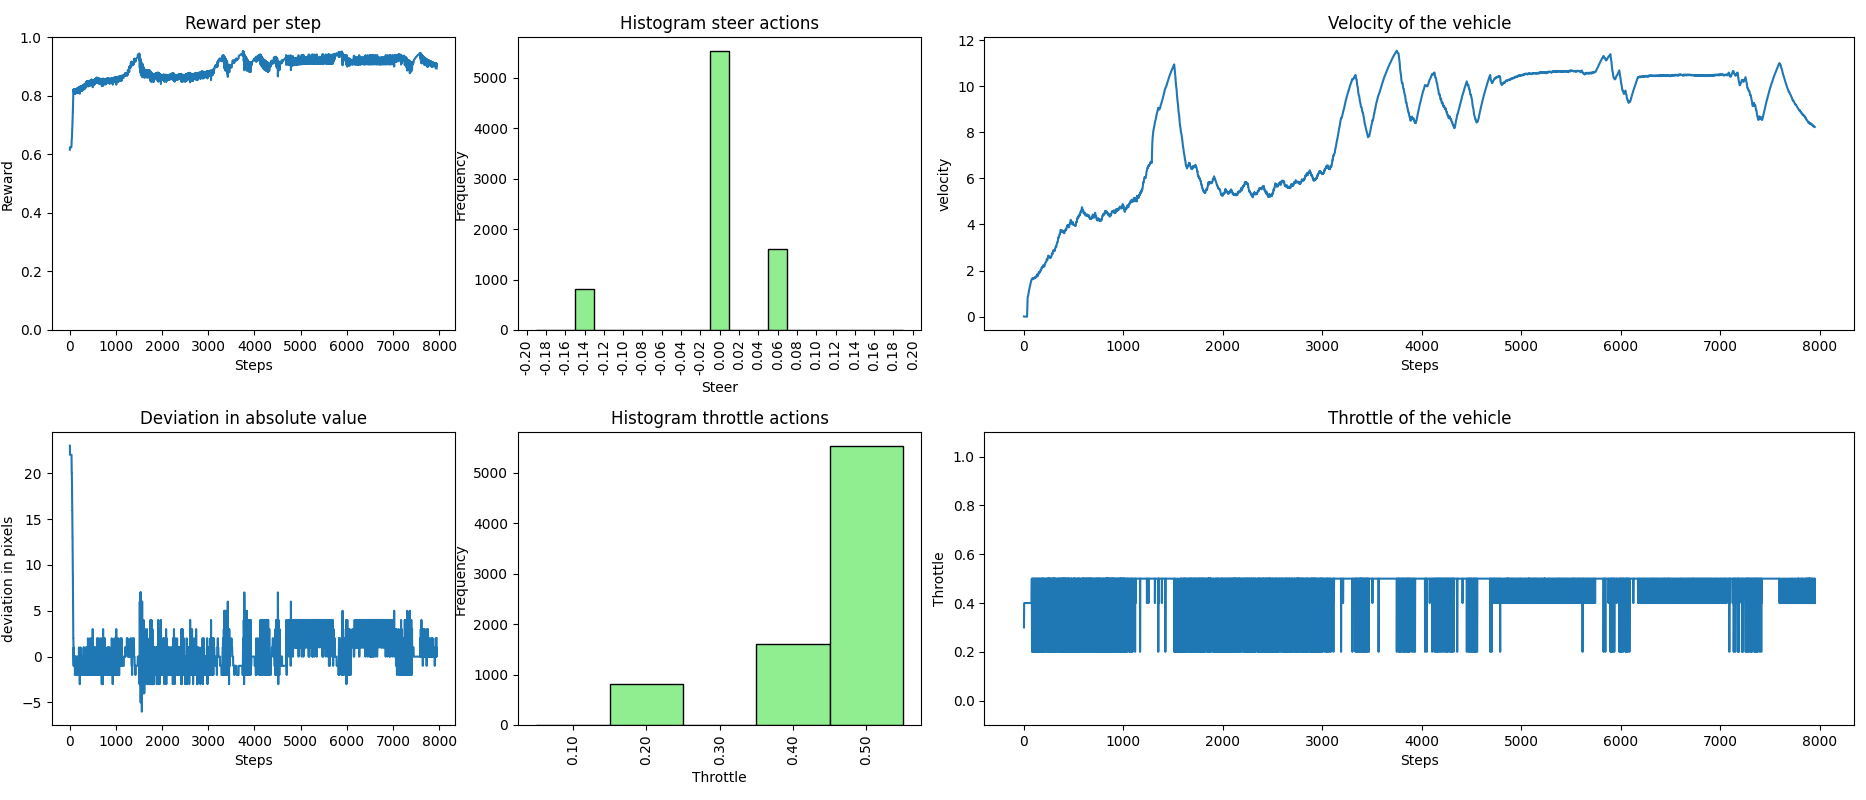
\includegraphics[width=\textwidth]{figs/Diseño/discrete/inference_dqn.png}
\caption{Histogramas de las acciones escogidas en inferencia por el modelo sigue-carril basado en \ac{DQN}.}
\label{fig:inference_dqn}
\end{figure}

En la Figura \ref{fig:comparativa_dqn}, se muestra la velocidad del coche autónomo en m/s y el error al centro del carril en píxeles del modelo basado en \ac{DQN} durante dos minutos, comparando un escenario visto durante el entrenamiento\footnotemark[3], con otro circuito no visto previamente\footnote{\url{https://youtu.be/QT0PQfs9-m8}}. Debemos tener en cuenta que el circuito de entrenamiento, identificado como circuito 1 en la Figura \ref{fig:mapa}, presenta curvas más abiertas en comparación con el nuevo circuito, descrito en la Figura \ref{fig:cir3}. A pesar de estas diferencias, en ambos casos, el histograma correspondiente a la desviación del carril se mantiene centrado, hecho que con el controlador \ac{PID} no sucedía. Esto indica que el modelo es capaz de generalizar y seguir el carril con precisión, incluso cuando el entorno cambia. En el circuito no entrenado, debido a las curvas más pronunciadas, la velocidad disminuye para garantizar una conducción segura.

\begin{figure}[ht]
\centering
\subfigure[Histogramas de un circuito visto durante el entrenameinto (Town03).]{\includegraphics[width=0.45\textwidth]{figs/Diseño/discrete/train_env.png} \label{fig:pid_ajus}}
\hfill
\subfigure[Histogramas de un circuito no visto durante el entrenamiento (Town04).]{\includegraphics[width=0.45\textwidth]{figs/Diseño/discrete/no_train_env.png} \label{fig:pid_no_ajus}}
\caption{Comparativa de la velocidad y desviación del carril del modelo basado en \ac{DQN}.}
\label{fig:comparativa_dqn}
\end{figure}
\newpage

Si comparamos este comportamiento con el obtenido en el controlador \ac{PID}, descrito en la sección \ref{fig:comparativa_pid}, vemos que, aunque el modelo basado en \ac{DQN} puede alcanzar velocidades superiores, generalmente es más lento. No obstante, se observa una mejora significativa en el seguimiento preciso del carril, especialmente en el escenario no ajustado o no visto durante el entrenamiento. Como se observa en el histograma \ref{fig:comparativa_dqn}(b), el modelo basado en \ac{DQN} es capaz de generalizar y mantenerse dentro de los límites del carril en todo momento con mayor precisión, garantizando una conducción más segura incluso en escenarios nuevos. En este caso, la desviación estándar respecto al centro del carril durante todo el circuito es de 2,6 píxeles. Por el contrario, el controlador \ac{PID}, como se muestra en el histograma \ref{fig:comparativa_pid}(b), presenta desviaciones mucho mayores en el circuito no ajustado, con una desviación estándar de 13.5 píxeles durante el recorrido, proporcionando un seguimiento de carril más inestable e inseguro.

Para analizar el rendimiento del sistema, se ha llevado a cabo un \textit{profiling} que permite evaluar tanto el tiempo dedicado a la detección del carril, como el tiempo que \ac{DQN} emplea para seleccionar la mejor acción a partir de las observaciones dadas. Este tiempo es mínimo, aunque superior al del controlador tradicional \ac{PID}. Esto se debe a que el modelo basado en \ac{DQN} requiere una fase de inferencia en la red neuronal, añadiendo un ligero coste computacional en comparación con las operaciones algebraicas simples del controlador \ac{PID}. Si sumamos el tiempo de decisión (1.25 ms) con el coste de percepción (10.75 ms), obtenemos una latencia total en torno a los 12 ms. La diferencia respecto al comportamiento basado en el controlador \ac{PID} es de 1-2 ms, por lo que el sistema sigue siendo totalmente apto para aplicaciones en tiempo real. Aunque nuestro sistema puede operar a aproximadamente 83 \ac{FPS} en inferencia, como se muestra en el vídeo anterior\footnotemark[3], conseguimos ejecutar CARLA a una tasa de 60-62 \ac{FPS}. Esto se debe a la carga computacional adicional introducida por los procesos de renderizado, el modelo de físicas del vehículo y otros cálculos necesarios para la simulación.

\subsection{Seguimiento de carril basado en PPO}

El objetivo sigue siendo conseguir un seguimiento de carril fluido a velocidades óptimas, pero esta vez usamos el algoritmo \ac{PPO}, que permite tanto un espacio de observaciones como de acciones continuo, lo cual es lo idóneo para nuestro entorno de conducción autónoma y futuros escenarios donde proponemos realizar adelantamiento seguro. El modelo podrá elegir la combinación de acelerador y giro idónea para cada momento, sin limitarse a pares predefinidos como ocurría con \ac{DQN}. Se emplea la misma lógica para terminar un episodio, sensores, \textit{fixed\_delta\_seconds} de 50 ms y circuito de entrenamiento que el modelo basado en \ac{DQN}, mostrado en la Figura \ref{fig:mapa}. Seguimos controlando dos actuadores: el acelerador y el giro. Se permite todo el rango del acelerador [0.0, 1.0], pero se limita el rango del giro a [-0.2, 0.2], ya que al entrenar el modelo basado en \ac{DQN} comprobamos que este intervalo era suficiente para completar el circuito con éxito y de forma precisa. Esto agiliza los entrenamientos y facilita la convergencia del modelo.

\begin{code}[h]
\begin{lstlisting}[language=Python]
self._max_steer = 0.2
self.action_space = spaces.Box(
    low=np.array([0.0, -self._max_steer]),
    high=np.array([1.0, self._max_steer]),
    shape=(2,),
    dtype=np.float64
)
\end{lstlisting}
\caption[Espacio de acciones sigue-carril basado en \ac{PPO}]{Espacio de acciones sigue-carril basado en \ac{PPO}.}
\label{cod:acc_ppo}
\end{code}

Sin embargo, se han llevado a cabo algunos cambios en las observaciones. Se ha añadido la velocidad actual del vehículo para mejorar la comprensión de la función de recompensa. En lugar de cinco, ahora el modelo recibe diez puntos de cada línea del carril, como se muestra en la Figura \ref{fig:puntos_carril_ppo}, para mejorar la comprensión del mismo sobre todo en las curvas.
\begin{figure}[ht]
\centering
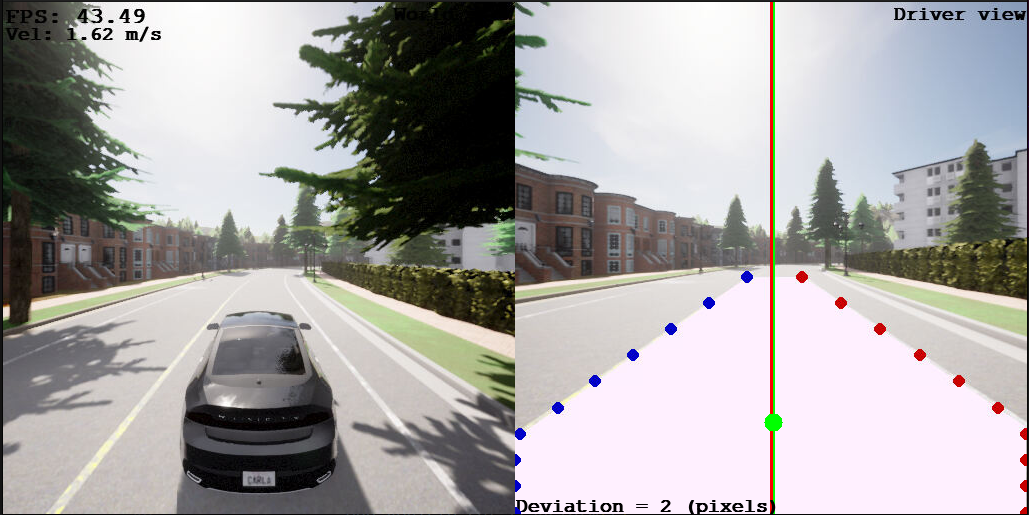
\includegraphics[width=9cm]{figs/Diseño/cont/lane10.png}
\caption{Observaciones sigue-carril basado en \ac{PPO}.}
\label{fig:puntos_carril_ppo}
\end{figure}

\newpage

En este caso, la función recompensa es más compleja y sigue el esquema descrito en la Figura \ref{fig:esquema_PPO}:

\begin{figure}[ht]
\centering
\includegraphics[width=\textwidth]{figs/Diseño/cont/diagrama.jpg}
\caption{Esquema de la función de recompensa del sigue-carril basado en \ac{PPO}.}
\label{fig:esquema_PPO}
\end{figure}

\begin{enumerate}
\item \textit{Comprobación de errores:} Primero se verifica si ha ocurrido un error, como la pérdida del carril o el choque contra elementos de la carretera. Si ocurre, se finaliza el episodio y se asigna una recompensa negativa.
\item \textit{Normalización lineal de elementos:} Si no hay errores, se normalizan los elementos de los que depende la recompensa:
\begin{itemize}
\item \textit{Desviación:} Se limita el valor de la desviación en el rango de [-100, 100] píxeles. Se lleva a cabo una normalización inversamente proporcional, cuanto mayor sea el error al centro del carril menor es la recompensa proporcionada.
\item \textit{Giro:} Para giros bruscos, en los rangos [-0.2, -0.14] o [0.14, 0.2], la recompensa es nula. En cambio, para giros no bruscos, dentro del límite [-0.14, 0.14], de nuevo la recompensa se normaliza inversamente, donde giros menores otorgan mayor recompensa.
\item \textit{Acelerador:} Si las aceleraciones son bruscas, en el rango [0.6, 1.0], la recompensa es nula. Para aceleraciones no bruscas, en la franja [0.0, 0.6), se normaliza de forma que mayores aceleraciones otorgan mayor recompensa. Sin embargo, si se excede una velocidad máxima, en este caso de 45 m/s, el acelerador se normaliza inversamente, valores más bajos proporcionan mayor recompensa.
\end{itemize}

\item \textit{Asignación de pesos a los elementos:} Finalmente, se define el peso de cada elemento en la recompensa según los siguientes criterios:
\begin{itemize}
\item Si el giro o el acelerador son bruscos, tienen un peso muy elevado en la recompensa, mientras que los otros dos elementos tienen un peso mucho menor.
\item Si se supera la velocidad máxima, el acelerador tiene mayor peso para intentar decelerar. También se penaliza bastante girar el volante, ya que a altas velocidades puede tener un gran impacto.
\item Si el acelerador es bajo, en el rango [0.0, 0.5), se penalizan menos los giros grandes, facilitando las curvas al reducir la velocidad.
\item Por el contrario, si el acelerador está en un rango moderado [0.5, 0.6), se penalizan más los giros grandes, enfocándose en zonas rectas o con giros leves.
\end{itemize}
\end{enumerate}

  \begin{myequation}[h]
    \begin{equation} 
      \text{reward} = w_{\text{dev}} \cdot r_{\text{dev}} + w_{\text{throttle}} \cdot r_{\text{throttle}} + w_{\text{steer}} \cdot r_{\text{steer}}
    \end{equation} 
    \caption{Función de recompensa para el sigue-carril basado en \ac{PPO}.}
\label{eq:rew_ppo}
  \end{myequation}

\begin{code}[H]
\begin{lstlisting}[language=Python]
if error == None:
    # Deviation normalization
    r_dev = (MAX_DEV - abs(np.clip(self._dev, -MAX_DEV, MAX_DEV))) / MAX_DEV

    # Steer conversion
    limit_steer = 0.14
    if abs(self._steer) > limit_steer:
        r_steer = 0
    else:
        r_steer = (limit_steer - abs(self._steer)) / limit_steer

    # Throttle conversion
    limit_throttle = 0.6
    if self._throttle >= limit_throttle:
        r_throttle = 0
    elif self._velocity > self._max_vel:
        r_throttle = (limit_throttle - self._throttle) / limit_throttle
    else:
        r_throttle = self._throttle / limit_throttle

    # Set weight
    if r_steer == 0: # Steer in range [-0.2, -0.14] or [0.14, 0.2]
        w_dev, w_throttle, w_steer = 0.1, 0.1, 0.8
    elif r_throttle == 0: # Throttle in range [0.6, 1.0]
        w_dev, w_throttle, w_steer = 0.1, 0.8, 0.1
    elif self._velocity > self._max_vel:
        w_dev, w_throttle, w_steer = 0.1, 0.65, 0.25
    elif self._throttle < 0.5: # Throttle in range [0.0, 0.5)
        w_dev, w_throttle, w_steer = 0.65, 0.25, 0.1
    else:  # Throttle in range [0.5, 0.6)
        w_dev, w_throttle, w_steer = 0.6, 0.15, 0.25

    reward = w_dev * r_dev + w_throttle * r_throttle + w_steer * r_steer
else:
    reward = -40
\end{lstlisting}
\caption[Función de recompensa para sigue-carril basado en \ac{PPO}]{Función de recompensa para sigue-carril basado en \ac{PPO}.}
\label{cod:rew_ppo}
\end{code}

De manera similar a lo que ocurría en el entrenamiento anterior, los hiperparámetros \textit{n\_steps} y el tamaño del lote fueron clave a la hora de adquirir convergencia. Valores bajos de \textit{n\_steps} provocan que los ejemplares en cada actualización estén demasiado correlacionados dificultando la convergencia del modelo. Por otro lado, si el número de experiencias utilizado para cada actualización es pequeño, genera un gradiente más ruidoso y menos confiable que provoca inestabilidad en el entrenamiento. Finalmente, estos fueron los hiperparámetros de entrenamiento utilizados:
\begin{table}[ht]
\centering
\begin{tabular}{|l|l|p{9cm}|}
\hline
\textbf{Hiperparámetro} & \textbf{Valor} & \textbf{Descripción} \\ \hline
n\_steps & 512 & Número de pasos a ejecutar antes de cada actualización \\ \hline
batch\_size & 512 & Tamaño del lote utilizado para el entrenamiento: número de experiencias con las que se calcula el gradiente \\ \hline
ent\_coef & 0.1 & Coeficiente de entropía: controla el equilibrio entre la exploración y la explotación \\ \hline
n\_timesteps & 4,000,000 & Número total de \textit{steps} para el entrenamiento \\ \hline
\end{tabular}
\caption{Hiperparámetros de entrenamiento para el sigue-carril basado en \ac{PPO}.}
\label{tab:hiper_params_ppo}
\end{table}

\newpage

No obstante, el parámetro que tuvo un mayor impacto en la obtención de un comportamiento eficiente fue el coeficiente de entropía. Cuando sus valores eran bajos, el agente apenas exploraba el entorno, limitándose a explotar las primeras acciones que había probado, lo que conllevó en una solución ineficaz. Durante los primeros entrenamientos, con un coeficiente de entropía muy bajo (0.01), el agente siempre se decantaba por las acciones extremas dentro de los límites definidos como correctos, tanto para el acelerador ([0.0, 0.6]) como para el giro ([-0.14, 0.14]). Combinado con estos dos factores, el vehículo se quedaba completamente inmóvil o rápidamente se salía del carril. Posteriormente, aumentado su valor, se logró regular el acelerador, pero el agente continuaba eligiendo las acciones extremas para el giro, lo que resultó en un comportamiento de péndulo. El agente ajustaba continuamente el ángulo de giro de manera excesiva, yendo constantemente de un lado a otro, provocando un comportamiento oscilante e ineficaz.

Para evaluar el equilibrio entre exploración y explotación durante el entrenamiento, se desarrolló un programa para analizar la frecuencia de las acciones tomadas. Finalmente, tras numerosas pruebas y análisis, se determinó que valores dentro del rango [0.08, 0.1] para el coeficiente de entropía eran los más óptimos para nuestra aplicación. En el gráfico \ref{fig:actions_ppo_carril}, se muestran los histogramas de estas acciones, donde se observa que finalmente ambas distribuciones están centradas, indicando que el modelo ha aprendido que las mejores acciones son giros suaves y aceleraciones moderadas, permitiendo alcanzar velocidades significativas sin excederse. Esto garantiza una conducción segura y precisa dentro del carril.

\begin{figure}[ht]
  \centering
  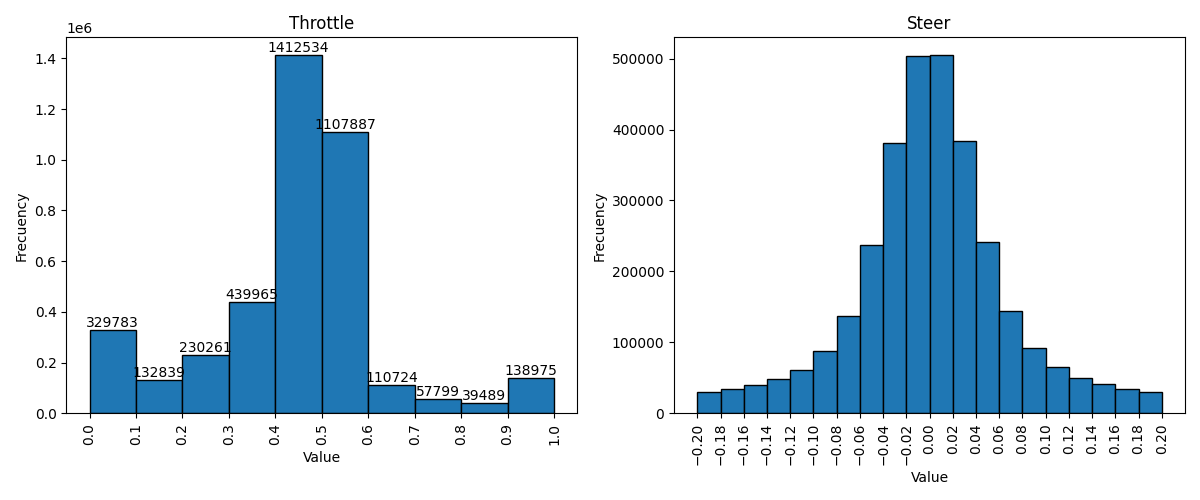
\includegraphics[width=13cm]{figs/Diseño/cont/actions.png}
  \caption{Histogramas de acciones tomadas durante el entrenamiento sigue-carril basado en \ac{PPO}.}
  \label{fig:actions_ppo_carril}
\end{figure}

\newpage

Los entrenamientos con \ac{PPO} duraron aproximadamente unas 20 horas. En el gráfico \ref{fig:train_ppo_carril}, se muestran los datos de entrenamiento del modelo sigue-carril basado en \ac{PPO}. El último \textit{plot} muestra la evolución de la velocidad media en cada episodio. Podemos observar cómo se logra rápidamente la convergencia, pero se necesitan más \textit{steps} para alcanzar velocidades significativas.
\begin{figure}[ht]
\centering
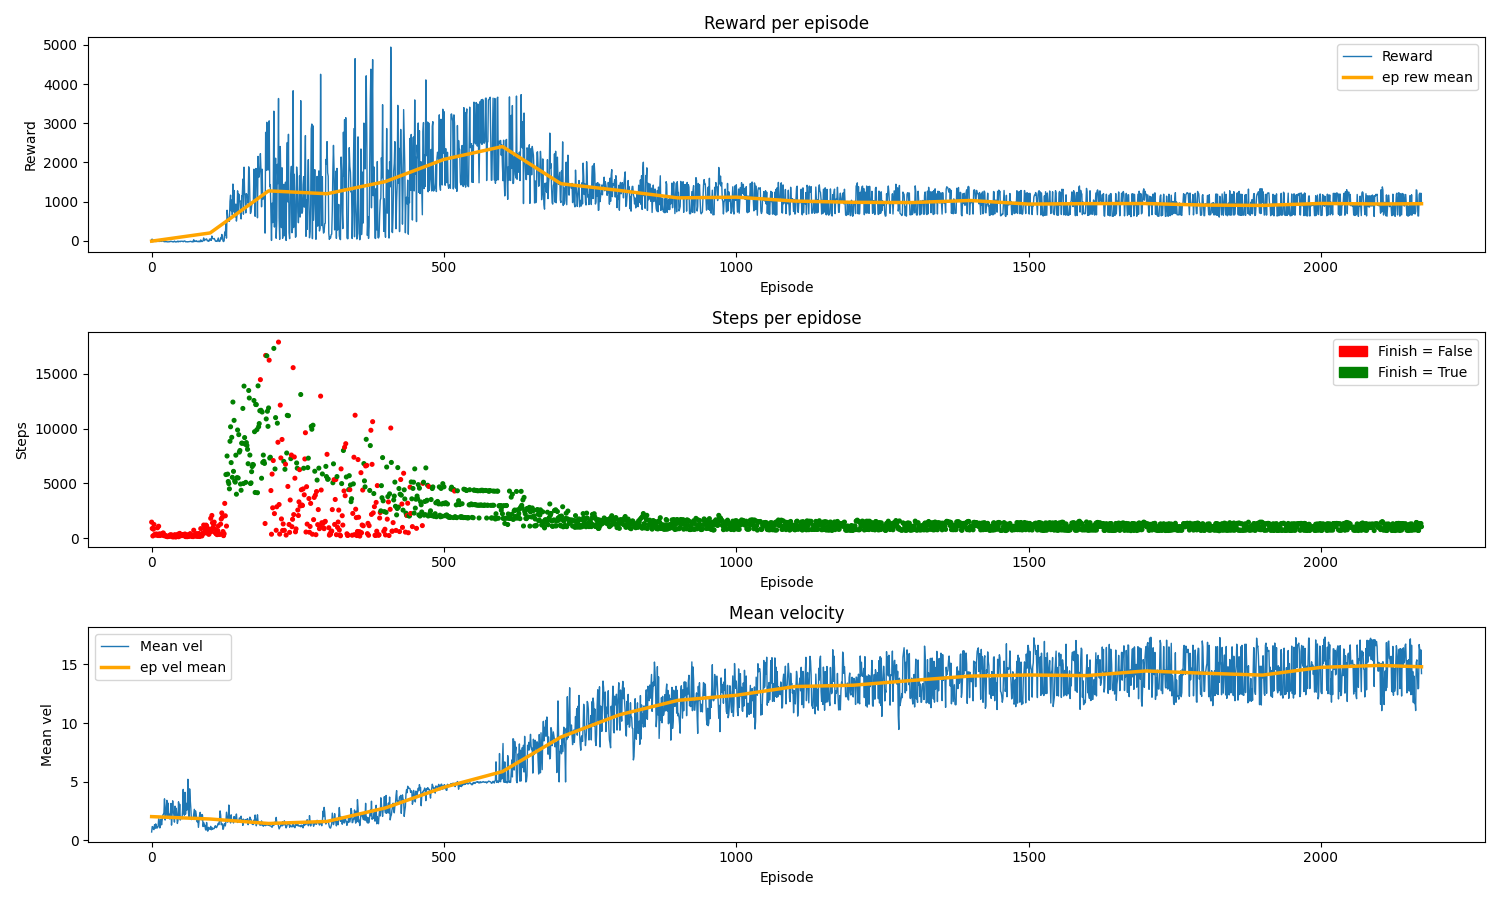
\includegraphics[width=\textwidth]{figs/Diseño/cont/train_ppo_carril.png}
\caption{Gráficas de entrenamiento sigue-carril basado en \ac{PPO}.}
\label{fig:train_ppo_carril}
\end{figure}

En inferencia obtenemos muy buenos resultados tanto en circuitos vistos durante el entrenamiento\footnote{\url{https://youtu.be/bZNfUwP14gc}} como en nuevos\footnote{\url{https://youtu.be/WRPLzKqJdto}}, incluso cambiando la ciudad en el simulador CARLA. Como reflejan los histogramas de la Figura \ref{fig:inference_ppo_carril}, el modelo siempre elige aceleraciones en el rango moderado [0.5, 0.6), combinadas con giros sutiles.
\begin{figure}[ht]
\centering
\includegraphics[width=13cm]{figs/Diseño/cont/inference.png}
\caption{Histogramas de las acciones escogidas en inferencia en un circuito de entrenamiento por el modelo sigue-carril basado en \ac{PPO}.}
\label{fig:inference_ppo_carril}
\end{figure} 

A diferencia del modelo basado en \ac{DQN}, ahora el agente puede elegir la combinación de acciones más óptima al disponer de un espacio de acciones continuo. Esto le permite seleccionar el giro exacto necesario en cada momento, alcanzando velocidades significativamente superiores en comparación con los modelos basados en \ac{DQN} y en el controlador \ac{PID}, descritos en las secciones \ref{fig:comparativa_dqn} y \ref{fig:comparativa_pid}, respectivamente. Además, es capaz de generalizar de manera más efectiva que los modelos previamente mencionados. Como se observa en la Figura \ref{fig:comparativa_ppo}, no se produce un deterioro en el rendimiento al cambiar de un escenario conocido (circuito 1 de la Figura \ref{fig:mapa}) a otro desconocido (mapa de la Figura \ref{fig:cir3}). Los datos han sido recopilados durante 40 segundos en ambos circuitos. Este enfoque da lugar a una conducción más fluida y segura, respetando con mayor precisión los límites del carril, tanto en escenarios vistos durante el entrenamiento como en nuevos entornos.

\begin{figure}[ht]
\centering
\subfigure[Histogramas de un circuito visto durante el entrenameinto (Town04).]{\includegraphics[width=0.45\textwidth]{figs/Diseño/cont/train_env.png} \label{fig:pid_ajus}}
\hfill
\subfigure[Histogramas de un circuito no visto durante el entrenamiento (Town03).]{\includegraphics[width=0.45\textwidth]{figs/Diseño/cont/no_train_env.png} \label{fig:pid_no_ajus}}
\caption{Comparativa de la velocidad y desviación del modelo sigue-carril basado en \ac{PPO} (percepción con \textit{ground thruth}).}
\label{fig:comparativa_ppo}
\end{figure}

\newpage

El modelo original aprendió con datos perfectos procedentes de \textit{ground truth}, pero si cambiamos la percepción del carril al modelo basado en \ac{DL}, el modelo se ajusta a trabajar con la salida de otra red neuronal, que puede introducir cierto ruido o variabilidad, intentando minimizar la brecha \textit{sim2real}. Este cambio también implica modificar la posición de la cámara, alterando la percepción visual. A pesar de estos ajustes, el modelo mantiene un seguimiento del carril fluido y preciso\footnote{\url{https://youtu.be/8kOpXYqzIGM}} sin reducir la velocidad en un circuito no visto durante el entrenamiento. Como se puede ver en la Figura \ref{fig:network_ppo_carril}, el histograma del error respecto al centro del carril permanece centrado. Esto demuestra la capacidad del modelo para adaptarse a nuevas condiciones, un aspecto clave en el desarrollo de sistemas de conducción autónoma robustos y confiables.
\begin{figure}[ht]
\centering
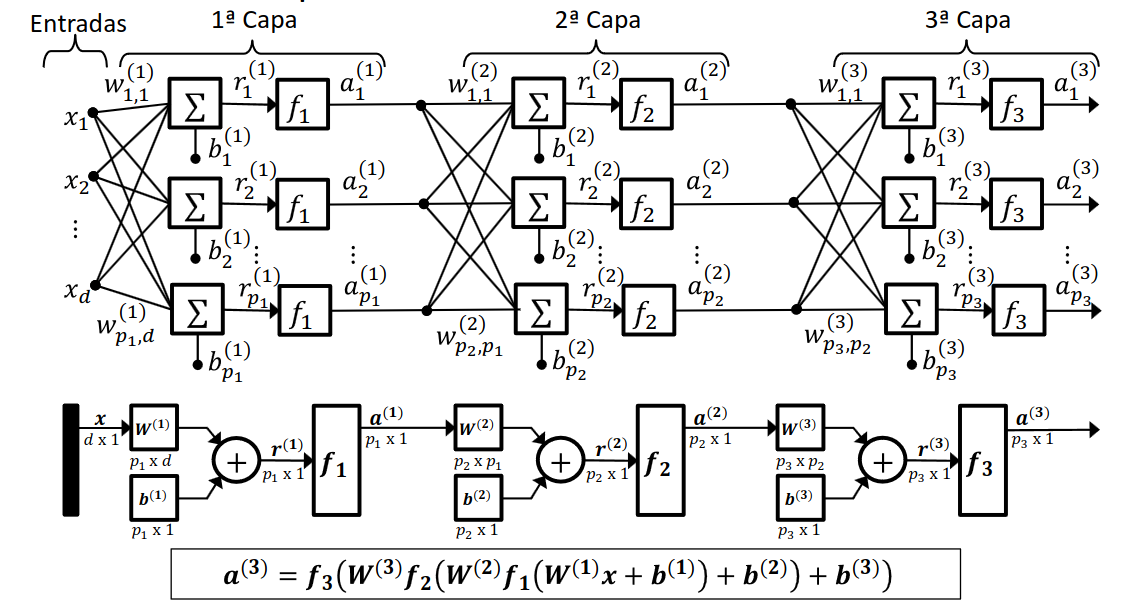
\includegraphics[width=9cm]{figs/Diseño/cont/network.png}
\caption{Datos de la velocidad y desviación del modelo sigue-carril basado en \ac{PPO} (percepción con el modelo basado en \ac{DL}) en un circuito no visto durante el entrenamiento (Town05). }
\label{fig:network_ppo_carril}
\end{figure}

Además, hemos probado el modelo en otros modelos de vehículos donde las dinámicas del vehículo cambian, como la masa, el torque, el centro de gravedad o la suspensión. Durante el entrenamiento se usó el modelo \textit{Lincoln MKZ 2017}, pero aun así los resultados obtenidos en otros modelos de coche\footnote{\url{https://youtu.be/oQyKaj4R6Js}}, motocicletas\footnote{\url{https://youtu.be/DRmLNmMDAms}} y furgonetas\footnote{\url{https://youtu.be/UE2OYPSaNWQ}} han sido igualmente muy satisfactorios. En la Figura \ref{fig:ppo_carril_din}, se muestran los datos de desviación respecto al centro del carril durante un circuito visto en el entrenamiento, donde todos los histogramas se mantienen centrados, indicando un seguimiento preciso del carril incluso cuando las dinámicas del vehículo cambian. Estos experimentos evidencian la gran capacidad de generalización del modelo, demostrando su eficacia en una amplia variedad de escenarios y configuraciones.
\begin{figure}[ht]
\centering
\begin{minipage}{0.32\textwidth}
    \centering
    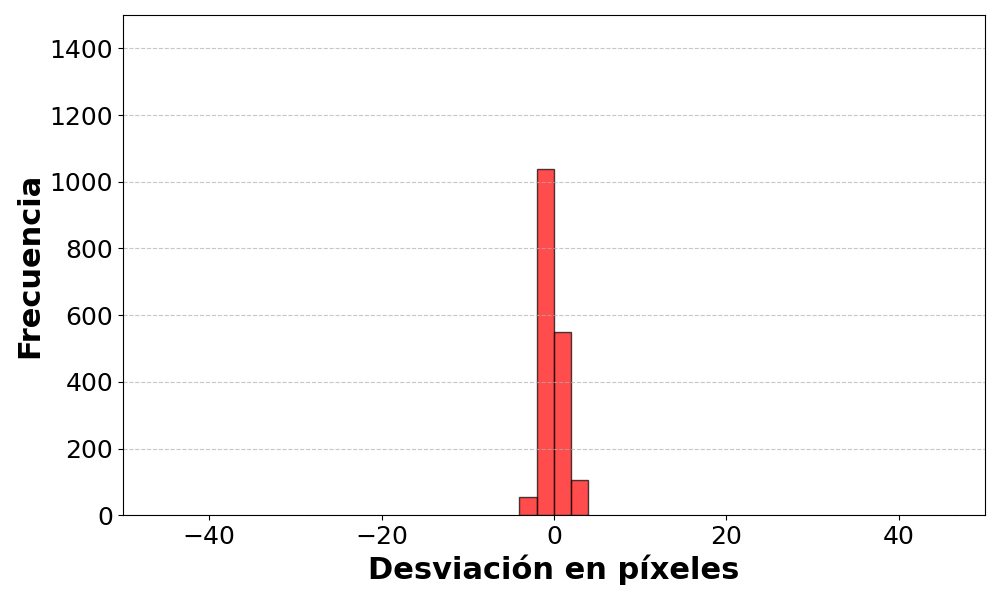
\includegraphics[width=\textwidth]{figs/Diseño/cont/otro.png}
    \caption{Otro modelo}
\end{minipage}%
\begin{minipage}{0.32\textwidth}
    \centering
    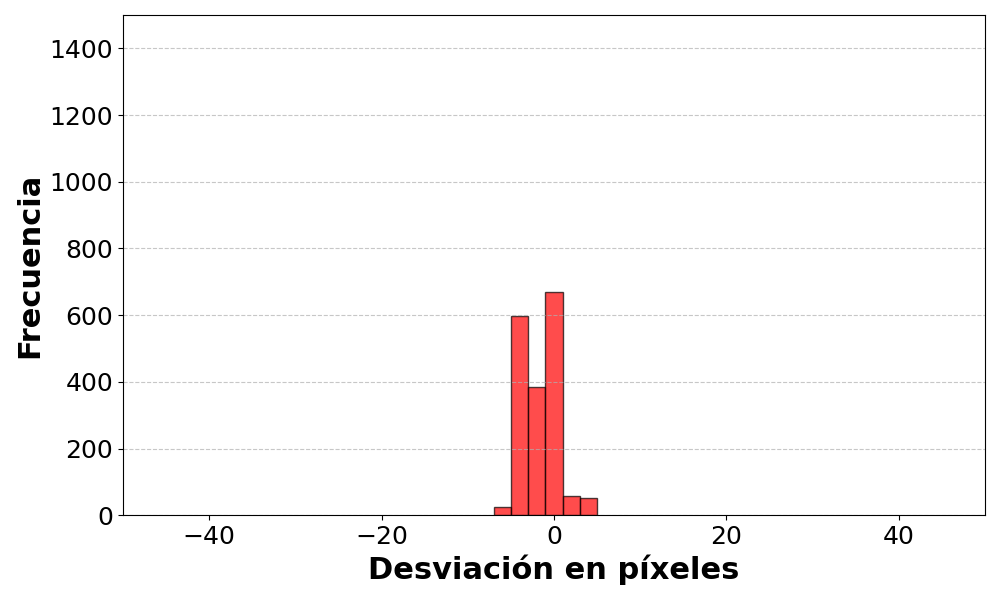
\includegraphics[width=\textwidth]{figs/Diseño/cont/furgoneta.png}
    \caption{Furgoneta}
\end{minipage}%
\begin{minipage}{0.32\textwidth}
    \centering
    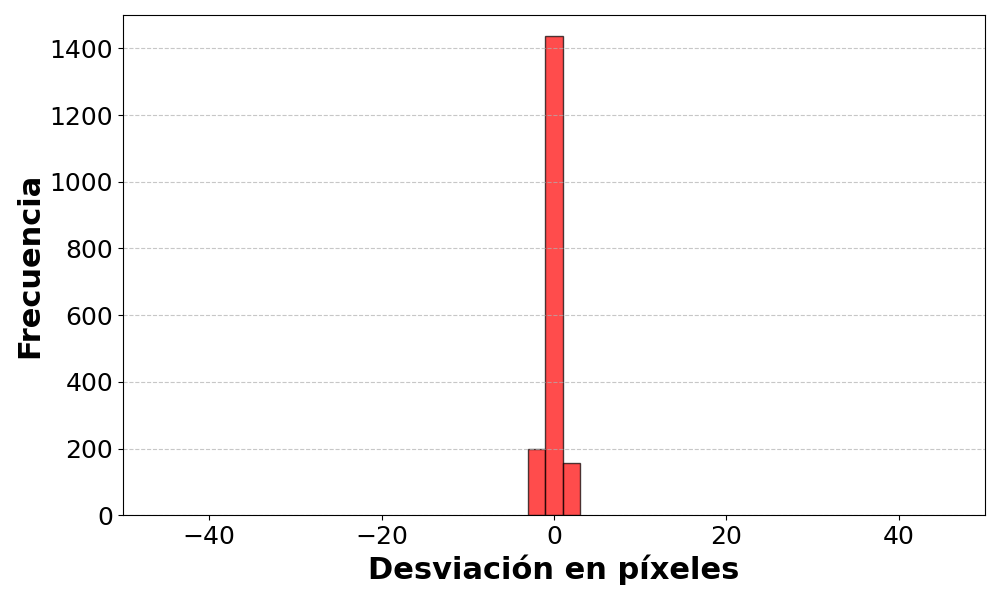
\includegraphics[width=\textwidth]{figs/Diseño/cont/moto.png}
    \caption{Motocicleta}
\end{minipage}
\caption{Desviación al centro del carril del modelo sigue-carril basado en \ac{PPO} en un circuito de entrenamiento (Town04) con otros vehículos (percepción \textit{ground truth}).}
\label{fig:ppo_carril_din}
\end{figure}

\newpage

\subsection{Control de crucero adaptativo basado en PPO}

Una vez que el coche sigue el carril de forma precisa y fluida, se define un nuevo objetivo. El vehículo autónomo debe ser capaz de regular su velocidad en función del vehículo que tiene delante. Para este nuevo comportamiento, necesitamos añadir un nuevo sensor, el \ac{LiDAR}. Mantenemos las mismas rutas de entrenamiento y seguimos utilizando el algoritmo de \ac{PPO} con el mismo espacio de acciones, ya que permite un mejor desempeño y adaptación al entorno. A las observaciones del modelo basado en \ac{PPO} para el seguimiento de carril, añadimos la información referente al \ac{LiDAR}. En este caso, se incorpora una única observación que incluye veinte puntos de la subzona frontal del \ac{LiDAR}, como se muestra en el Código \ref{fig:laser_front}.

\begin{code}[h]
\begin{lstlisting}[language=Python]
self._num_points_laser = 20
self.observation_space[KEY_LASER] = spaces.Box(
	low=MIN_DIST_LASER - 1.0,
	high=MAX_DIST_LASER,
	shape=(self._num_points_laser,),
	dtype=np.float64
)
\end{lstlisting}
\caption[Definición de observación frontal del \ac{LiDAR}]{Definición de observación frontal del \ac{LiDAR}.}
\label{cod:obs_laser_front}
\end{code}

Un cambio clave respecto al modelo anterior es que, esta vez, hemos entrenado a 10 \ac{FPS} en lugar de 20 \ac{FPS}. A 20 \ac{FPS}, el agente no lograba un comportamiento de crucero adaptativo eficiente, sino un efecto de \textit{muelle}, acercándose demasiado al coche de delante, frenando bruscamente, alejándose y repitiendo el ciclo. En cambio, a 10 \ac{FPS}, se ha conseguido un comportamiento más estable. Esto se debe a que, a velocidades bajas, las observaciones consecutivas no varían significativamente a 20 \ac{FPS}, lo que introduce redundancia en los datos y prolonga el entrenamiento. Reduciendo los \ac{FPS}, se optimiza el tiempo de aprendizaje sin afectar a la calidad de las decisiones del agente. Además, al tener más tiempo para reaccionar a los cambios, el agente puede tomar decisiones más suaves y precisas, evitando movimientos bruscos y mejorando la estabilidad general del comportamiento.

En este nuevo escenario, las observaciones han cambiado, por lo tanto, no podemos reutilizar el modelo anterior de seguimiento de carril basado en \ac{PPO}, pero sí sus parámetros y función de recompensa. Para facilitar el aprendizaje del modelo, hemos utilizado la estrategia de \textit{curriculum learning}. Consiste en presentar al modelo las tareas de manera progresiva, comenzando con las más simples e ir aumentando gradualmente la complejidad. Este enfoque imita la forma en que los humanos aprenden, empezando por conceptos básicos antes de abordar problemas más difíciles. Reducir la complejidad al inicio evita que el agente aprenda de manera irregular con grandes fluctuaciones en la política, mejorando la estabilidad del entrenamiento y aumentando la velocidad de convergencia. Además, al aprender de forma estructurada, el modelo tiende a desarrollar representaciones más sólidas que mejoran la generalización \cite{curriculum-learning}. Basándonos en la función de recompensa para el seguimiento de carril mediante \ac{PPO}, definida en el código \ref{cod:rew_ppo}, se ha diseñado la siguiente función de recompensa adaptada a este nuevo caso, en el que se incorporan las observaciones del \ac{LiDAR}, aunque estas no sean relevantes para este comportamiento.

  \begin{myequation}[h]
    \begin{equation} 
      \text{reward} = w_{\text{dev}} \cdot r_{\text{dev}} + w_{\text{throttle}} \cdot r_{\text{throttle}} + w_{\text{steer}} \cdot r_{\text{steer}} + w_{\text{lidar}} \cdot r_{\text{lidar}}
    \end{equation} 
    \caption{Función de recompensa para el control de crucero adaptativo basado en \ac{PPO}.}
\label{eq:rew_ppo_adp}
  \end{myequation}

\begin{code}[H]
\begin{lstlisting}[language=Python]
if r_steer == 0:
    w_dev, w_throttle, w_steer, w_lidar = 0.1, 0.1, 0.8, 0.0
elif r_throttle == 0:
    w_dev, w_throttle, w_steer, w_lidar = 0.1, 0.8, 0.1, 0.0
elif self._velocity > self._max_vel:
    w_dev, w_throttle, w_steer, w_lidar = 0.1, 0.65, 0.25, 0.0
else:
    w_dev, w_throttle, w_steer, w_lidar = 0.6, 0.2, 0.2, 0.0 # Follow Lane
\end{lstlisting}
\caption[Función de recompensa sigue-carril para el control de crucero adaptativo con \ac{PPO}]{Función de recompensa sigue-carril para el control de crucero adaptativo basado en \ac{PPO}.}
\label{cod:rew_carril_ppo_passing}
\end{code}

Se han preservado los valores de los hiperparámetros de entrenamiento utilizados en el comportamiento sigue-carril basado en \ac{PPO}, expuestos en la tabla \ref{tab:hiper_params_ppo}, exceptuando el coeficiente de entropía, el cual se ha reducido ligeramente a 0.08 para favorecer la explotación de acciones. El entrenamiento duró aproximadamente 28 horas y se obtuvieron resultados muy similares a los del apartado anterior, mostrados en la Figura \ref{fig:train_ppo_carril}. De nuevo, se consigue una convergencia total rápidamente, pero seguimos necesitando un número elevado de \textit{steps} para adquirir velocidades óptimas.

\begin{figure}[ht]
\centering
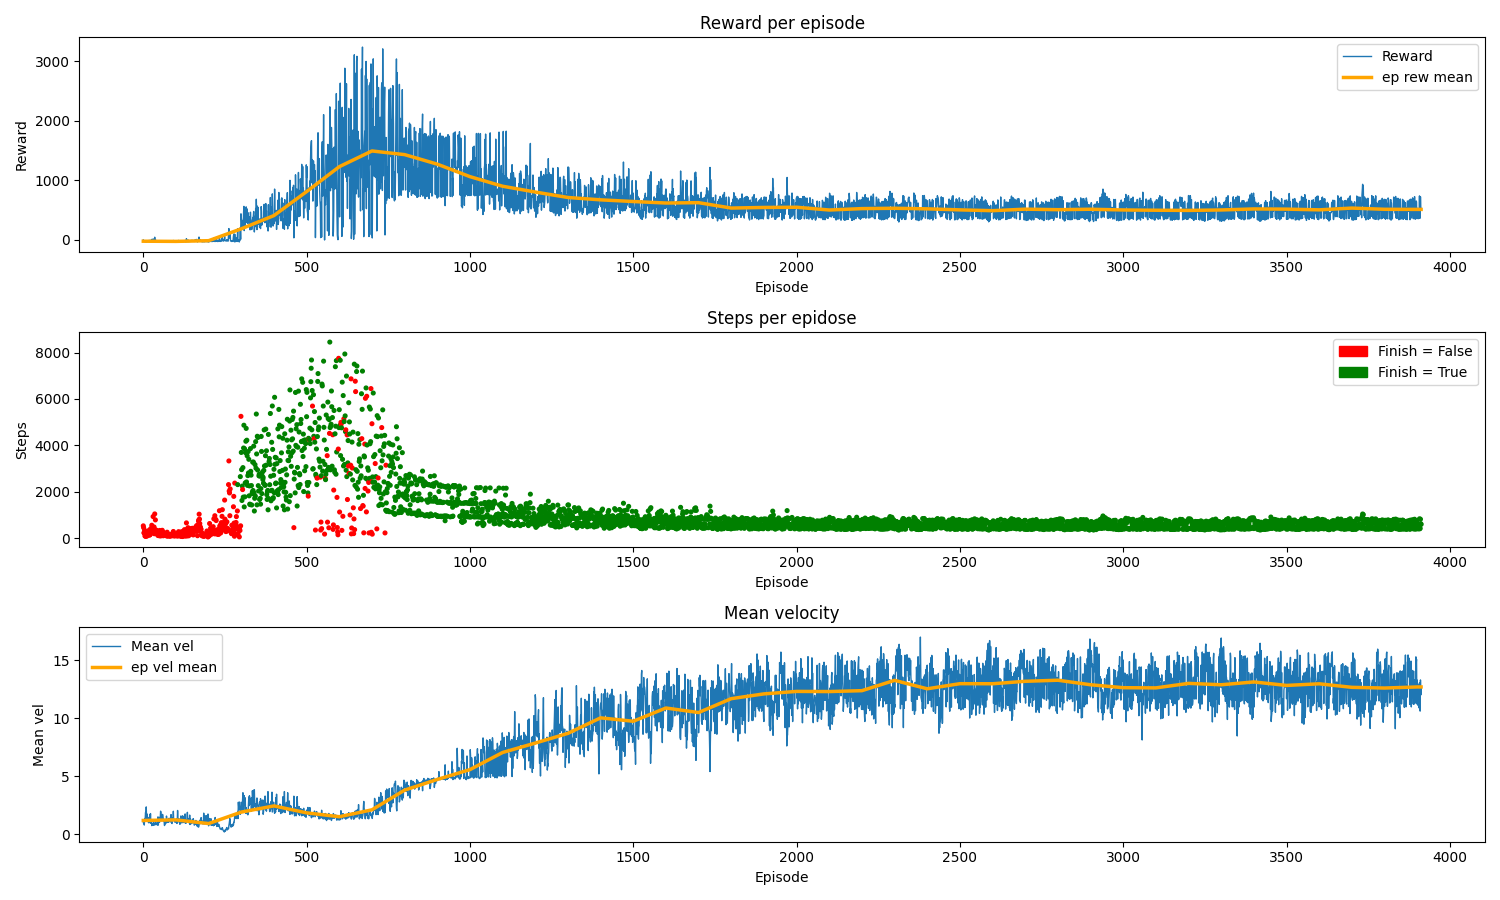
\includegraphics[width=\textwidth]{figs/Diseño/passing/train_base.png}
\caption{Datos de entrenamiento sigue-carril para el control de crucero adaptativo basado en \ac{PPO}.}
\label{fig:passing_train_base}
\end{figure}

El modelo adquirido sigue el carril de manera eficiente\footnote{\url{https://youtu.be/flTo3YyFCHU}} (el vídeo es un circuito de entrenamiento), eligiendo giros sutiles combinados con valores moderados del acelerador, en el rango de [0.47, 0.49]. Estos valores son ligeramente inferiores en comparación con el modelo sin el \ac{LiDAR}, ya que estas observaciones no son necesarias para el seguimiento de carril y solo aportan ruido al modelo. Aun así, obtenemos un modelo capaz de seguir el carril a la perfección en inferencia, alcanzando velocidades en torno a los 55 km/h. Además, la incorporación de un nuevo sensor incrementa la latencia total del sistema, reduciendo los \ac{FPS} a los que puede ejecutar el sistema.
\begin{figure}[ht]
\centering
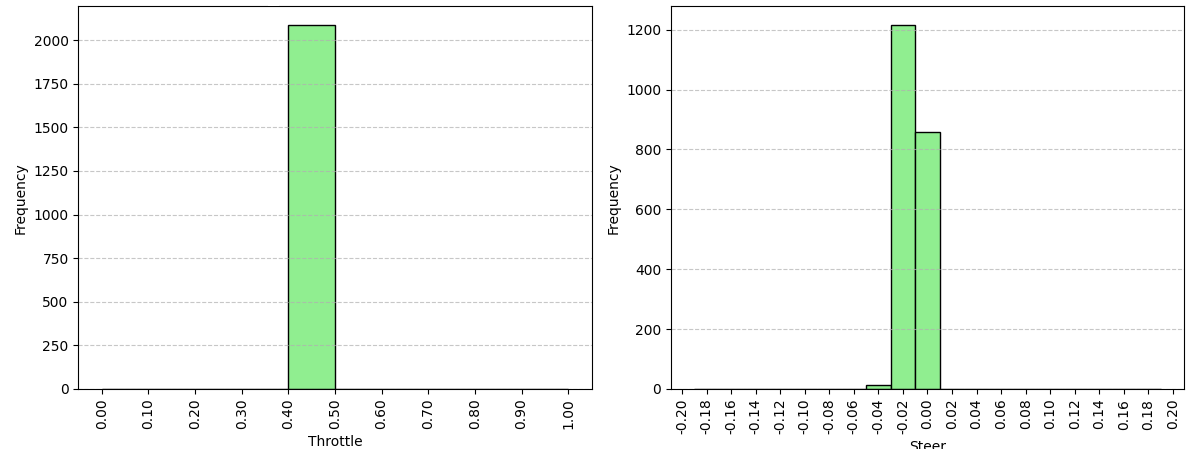
\includegraphics[width=14cm]{figs/Diseño/passing/actions_inference_base.png}
\caption{Histogramas de acciones tomadas en inferencia para el seguimiento del carril del modelo de control de crucero adaptativo basado en \ac{PPO} (Town04).}
\label{fig:passing_inference_lane}
\end{figure}

\newpage

Ahora, necesitamos reentrenar el modelo sigue-carril para lograr un control de crucero adaptativo respecto al vehículo delantero. Si la distancia medida por el \ac{LiDAR} es menor de 4 metros, se provoca una excepción y se finaliza el episodio dando una recompensa negativa. Esta acción se penaliza aún más que salirse del carril, puesto que es más grave y puede tener consecuencias fatales en el mundo real. Mientras no se obtengan medidas del \ac{LiDAR}, se aplica la recompensa asociada al seguimiento del carril. Sin embargo, si la distancia mínima captada por el \ac{LiDAR} está en el rango de 4 a 20 metros, esta medida se normaliza y se tiene en cuenta en la recompensa según se muestra en la Figura \ref{fig:diagrama_lidar}. Su peso depende de la distancia a la que el coche se sitúa del vehículo delantero: cuanto más próximo esté, mayor es su relevancia, puesto que aumenta la criticidad de la situación. Una vez detectamos el vehículo, el peso del acelerador disminuye drásticamente, deja de ser relevante ir a altas velocidades, el objetivo es no colisionar con el coche de delante y mantener la distancia de seguridad adecuada.

\begin{figure}[ht]
\centering
\includegraphics[width=\textwidth]{figs/Diseño/passing/diagrama.jpg}
\caption{Función de recompensa para el control de crucero adaptativo basado en \ac{PPO}.} \label{fig:diagrama_lidar}
\end{figure}

\begin{code}[H]
\begin{lstlisting}[language=Python]
if error == None:
    # Deviation normalization, Steer conversion and Throttle conversion

    # LiDAR conversion
    if self._passing and not np.isnan(self._dist_laser):
        r_lidar = (np.clip(self._dist_lidar, MIN_DIST_LIDAR, MAX_DIST_LIDAR) - MIN_DIST_LIDAR) / (MAX_DIST_LIDAR - MIN_DIST_LIDAR)       
    else:
        r_lidar = 0

    # Set weights
    # Filter inadequate actions
    elif r_lidar != 0:
        if self._dist_lidar <= 10:
            w_lidar, w_steer, w_dev, w_throttle = 0.9, 0.0, 0.1, 0.0
        elif self._dist_laser <= 12:
            w_lidar, w_dev, w_steer, w_throttle = 0.5, 0.45, 0.05, 0.0
        else:
            w_lidar, w_dev, w_steer, w_throttle = 0.4, 0.5, 0.05, 0.05
    # Follow lane

    reward = w_dev * r_dev + w_throttle * r_throttle + w_steer * r_steer + w_lidar * r_lidar
else:
    if "Distance" in error:
        reward = -60 # LiDAR error
    else:
        reward = -40 # Lane error
\end{lstlisting}
\caption[Función de recompensa respecto al \ac{LiDAR} para control de crucero adaptativo basado \ac{PPO}]{Función de recompensa respecto al \ac{LiDAR} para control de crucero adaptativo basado \ac{PPO}.}
\label{cod:rew_ppo_passing}
\end{code}

La elección de las velocidades a lo largo de cada episodio del vehículo delantero, controlado por el autopiloto de CARLA, fue crucial para lograr un comportamiento estable, pero también una tarea compleja. Es fundamental contar con escenarios en los que las condiciones del entorno se ajusten para asegurar que el modelo vea una amplia variedad de situaciones. Esto evita el sobreajuste a problemas específicos y fomenta la generalización, obteniendo un modelo más robusto y con mejor rendimiento.

A la hora de diseñar el escenario de entrenamiento, primero se intentó estableciendo una velocidad constante durante un periodo de entre 100 y 450 \textit{steps} en un rango de [5, 10] m/s, escogiendo valores enteros y ambos de manera aleatoria. Sin embargo, se obtenía un modelo muy lento, que como máximo alcanzaba velocidades de 7 m/s. Para detectar donde estaba el problema, calculamos durante que porcentaje del episodio el coche detectaba al vehículo delantero con el \ac{LiDAR}, así como la cantidad de \textit{steps} en los que se ha detectado el vehículo delantero en cada una de las velocidades durante el entrenamiento. El problema erradicaba en que, para velocidades altas, el vehículo delantero se alejaba demasiado, sin que el agente pudiera verlo en ningún momento, provocando el sobreajuste del modelo a velocidades bajas.

Para resolver esta situación, se diseñó un comportimento para que el vehículo delantero se detuviera si no estaba siendo detectado por el agente, pero, aun así, el modelo resultante seguía siendo demasiado lento. El porcentaje de detección era mayor del 80\% en todos los episodios. Por ello, se modificó este comportamiento para que el camión solo se detuviera a distancias superiores de 30 metros, la separación entre ambos vehículos se obtuvo directamente del simulador CARLA. De esta forma, garantizamos que el modelo pueda ver al vehículo delantero en todas las velocidades, a la vez que se generen ocasiones en las que no lo vea, lo que ayuda a evitar el sobreajuste del modelo y a mantener las altas velocidades. Finalmente, en la Figura \ref{fig:velocities}, se muestran los histogramas del número de \textit{steps} durante los que el agente ha observado las diferentes velocidades, así como aquellos en los que no ha detectado al vehículo delantero durante el reentrenamiento. La fracción de veces que ha detectado al vehículo delantero es muy superior a la que no lo detecta, pero debemos recordar que en el entrenamiento base de seguimiento de carril no ha visto un vehículo delante en ninguno de los episodios.

\begin{figure}[ht]
\centering
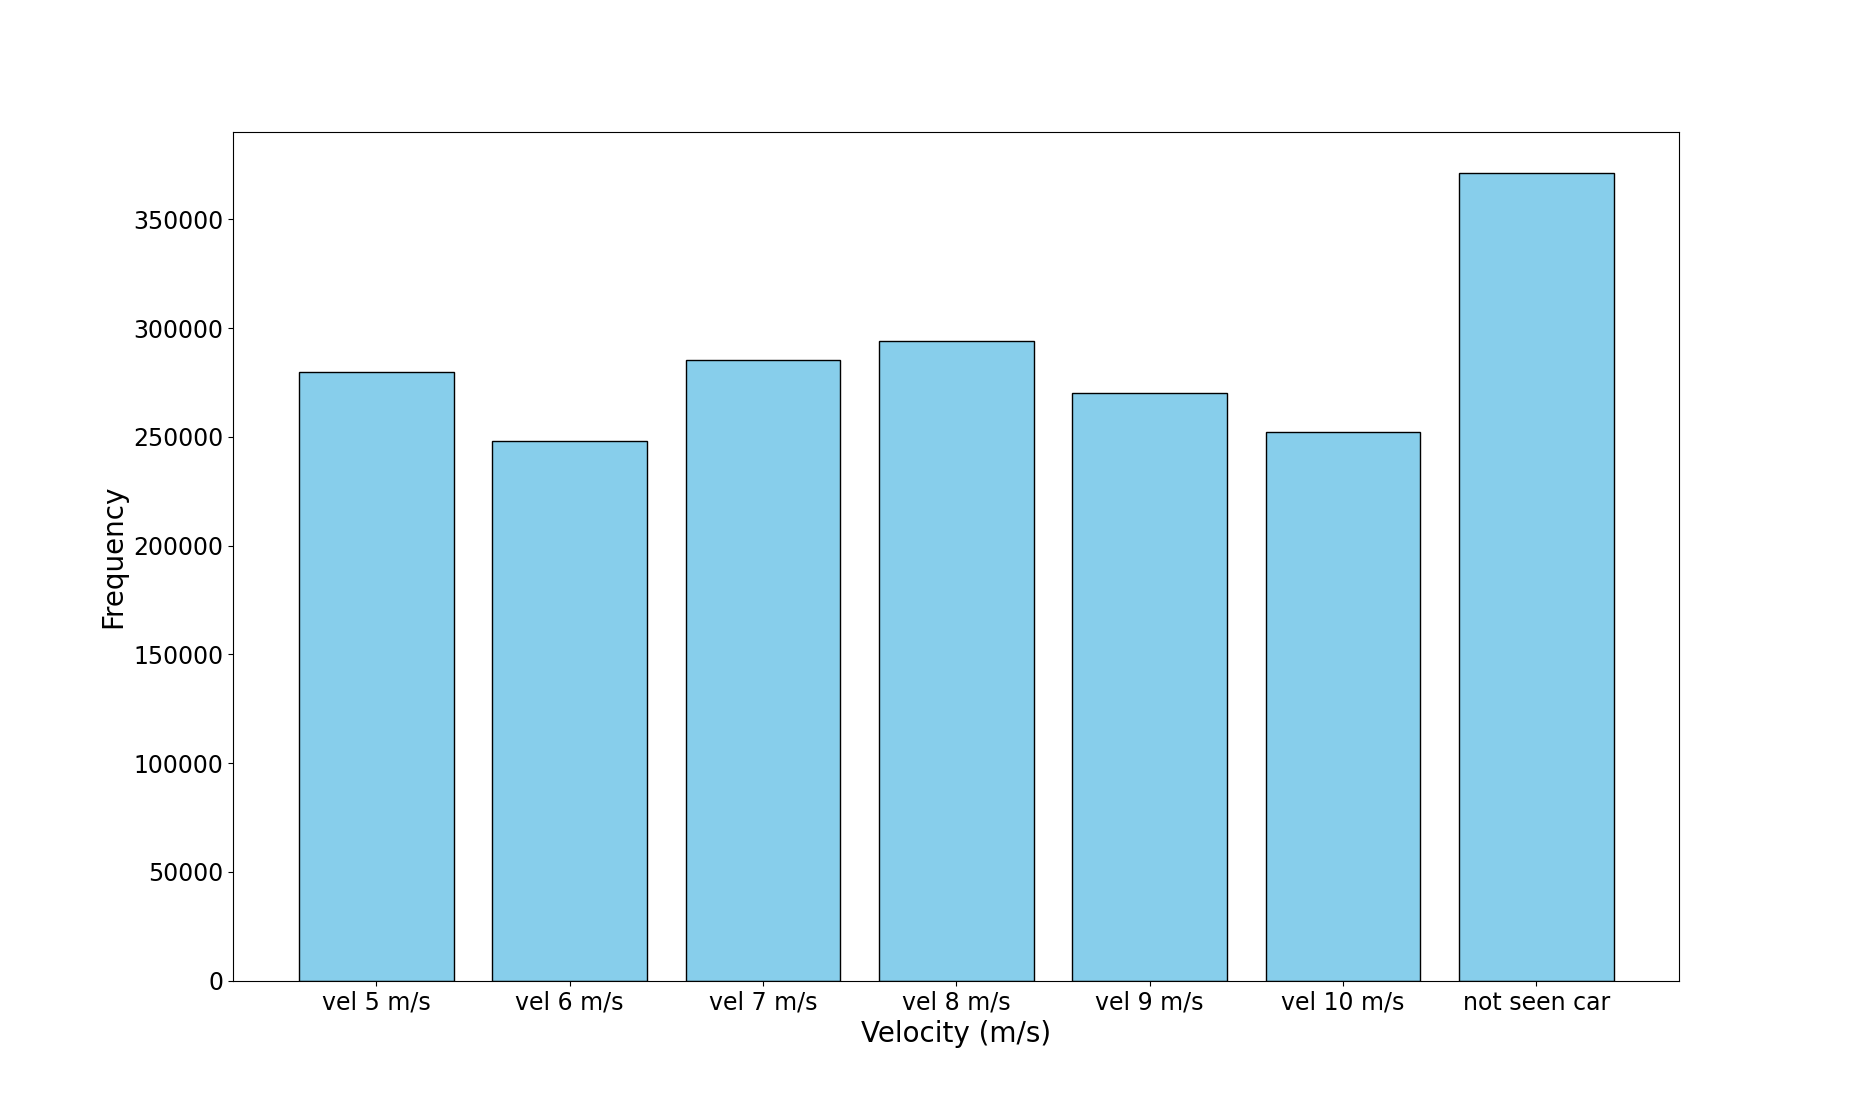
\includegraphics[width=12cm]{figs/Diseño/passing/velocities.png}
\caption{Histograma de velocidades del vehículo delantero vistas por el agente durante el entrenamiento para el control de crucero adaptativo basado en \ac{PPO}.}
\label{fig:velocities}
\end{figure}

Como el modelo ya ha aprendido a seguir el carril con una velocidad adecuada, no son necesarios tantos episodios de entrenamiento, por lo que hemos reducido el número total de \textit{steps} a la mitad. También se ha disminuido a la mitad el coeficiente de entropía (0.04), para agilizar el entrenamiento evitando escenarios poco probables. Los entrenamientos duraron aproximadamente 15 horas. En la Figura \ref{fig:train_traffic}, se puede ver que, aunque no se alcanza una convergencia total como en entrenamientos anteriores, podemos decir que el modelo sí converge, ya que la recompensa promedio de los episodios aumenta de manera progresiva a lo largo del proceso de entrenamiento. Esto sugiere que, a pesar de los episodios no finalizados (puntos rojos), el modelo está mejorando gradualmente su desempeño y aprendiendo de manera efectiva.
\begin{figure}[ht]
\centering
\includegraphics[width=\textwidth]{figs/Diseño/passing/train.png}
\caption{Datos del reentrenamiento del control de crucero adaptativo basado en \ac{PPO}.}
\label{fig:train_traffic}
\end{figure}

En la fase de inferencia, se obtienen buenos resultados a distintas velocidades, tanto altas\footnote{\url{https://youtu.be/mN0Y2q6ny5w}} como bajas\footnote{\url{https://youtu.be/Gvh9ZS0Sizc}}, y se mantiene el seguimiento preciso del carril. Los resultados son satisfactorios tanto en circuitos vistos durante el entrenamiento como nuevos, incluso cambiando de ciudad en CARLA\footnote{\url{https://youtu.be/ieMD1wqqEaY}} (Town06). A pesar de haber entrenado el modelo con un camión como vehículo delantero, también se adapta con éxito a otros modelos de coches\footnote{\url{https://youtu.be/RmD8-avcwvU}}, ambas pruebas evidencian la capacidad de generalización del modelo. En la Figura \ref{fig:infrence_passing}, se observa el histograma del acelerador elegido durante inferencia cuando el vehículo delantero circula a 9 m/s en un circuito de entrenamiento. La mayoría de acciones se concentran en el rango [0.4, 0.5], lo que sugiere que el coche mantiene una aceleración constante en lugar de realizar ajustes bruscos, logrando así una conducción más suave y eficiente.

\begin{figure}[ht]
\centering
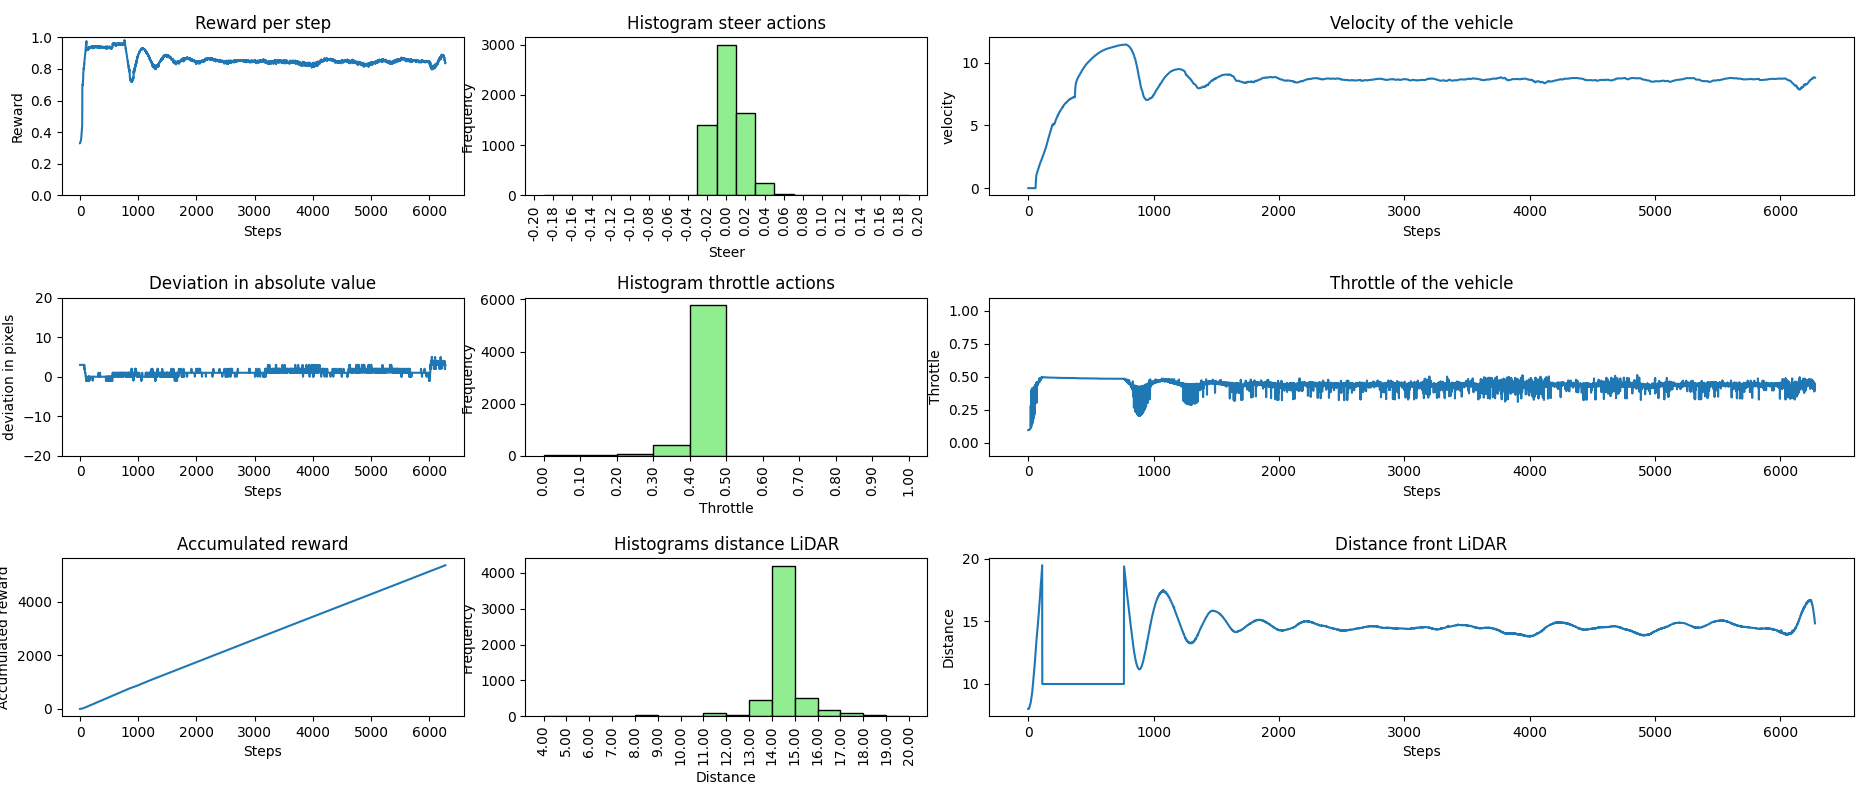
\includegraphics[width=7cm]{figs/Diseño/passing/inference_9.png}
\caption{Acelerador en inferencia del control de crucero adaptativo basado en \ac{PPO} a 9 m/s (Town04).}
\label{fig:infrence_passing}
\end{figure}

\newpage

La velocidad del coche delantero influye directamente en la distancia de estabilización, es decir, la separación con la que el coche autónomo se mantiene del vehículo delantero. A mayor velocidad, mayor es esta distancia de seguridad, lo que es lógico y necesario en un entorno real. Sin embargo, esta medida no es la distancia real que separa los vehículos, sino la distancia del \ac{LiDAR} al vehículo delantero, el cual está desplazado 0.5 metros hacia atrás con respecto al centro del coche. El modelo de coche usado tiene una longitud de aproximadamente 5 metros. Por lo tanto, para obtener la distancia real entre los vehículos, debemos restar 3 metros a las distancias medidas por el \ac{LiDAR}.

Tomando como referencia la regla del cuadrado\footnote{\url{https://www.caranddriver.com/es/movilidad/a40815294/distancia-de-seguridad-correcta-vehiculos/}} marcada por la \ac{DGT}, se ha calculado el percentil 90 para cada una de las velocidades, verificando que en todos los casos se respeta la distancia de seguridad recomendada. Por ejemplo, en el vídeo\footnotemark[12] observamos que, si el vehículo delantero se desplaza a 9 m/s, se mantiene una distancia de seguridad de 11-12 metros, mientras que la distancia mínima de seguridad marcada es de 10,5 metros.

Se ha llevado a cabo un \textit{profiling} para analizar el rendimiento del sistema ahora que hemos introducido un nuevo sensor, lo que claramente aumenta la latencia total. El tiempo de respuesta se duplica en comparación con el modelo sigue-carril basado en \ac{PPO}, pasando de 12 ms a 27 ms. Como resultado, la capacidad de ejecución de nuestro sistema se ha reducido a 37 \ac{FPS}, mientras que CARLA es capaz de ejecutar a 27-30 \ac{FPS}. A pesar de esta disminución en la velocidad de ejecución, sigue siendo suficiente para que el sistema reaccione eficientemente en tiempo real ante las diferentes situaciones planteadas.

\begin{figure}[ht]
\centering
\includegraphics[width=11cm]{figs/Diseño/passing/profiling.png}
\caption{\textit{Profiling} en inferencia del control de crucero adaptativo basado en \ac{PPO}.}
\label{fig:profiling_ppo_passing}
\end{figure}

\subsection{Maniobra de adelantamiento basada en PPO}

En este apartado se describe como se ha alcanzado el objetivo final, realizar una maniobra de adelantamiento completa. Esta maniobra comienza cuando el agenta detecta al vehículo delantero con el \ac{LiDAR}, y termina cuando ha regresado al carril inicial. Para ello, es necesario añadir nuevas observaciones al modelo, tanto referentes a la zona derecha del \ac{LiDAR}, como a la segmentación de la calzada con la red EfficientVit, descrita en la sección \ref{sec:per_ef}, con el fin de determinar si existe un carril al que desplazarse. Estas son todas las observaciones que recibe el modelo:
\begin{itemize}
\item Velocidad del propio agente, es decir, del \textit{Ego Vehicle}.
\item Desviación del carril.
\item Centro de masas del carril.
\item Área del carril.
\item 10 puntos de la línea de carril izquierda.
\item 10 puntos de la línea del carril derecha.
\item 10 puntos de la subzona frontal del \ac{LiDAR}.
\item 10 puntos de la subzona frontal derecha del \ac{LiDAR}.
\item 10 puntos de la subzona derecha del \ac{LiDAR}.
\item 10 puntos de la subzona trasera derecha del \ac{LiDAR}.
\item Centro de masas de la calzada.
\item Área de la calzada.
\item 16 puntos del límite izquierdo de la calzada.
\item 16 puntos del límite derecho de la calzada.
\end{itemize}

\begin{figure}[ht]
\centering
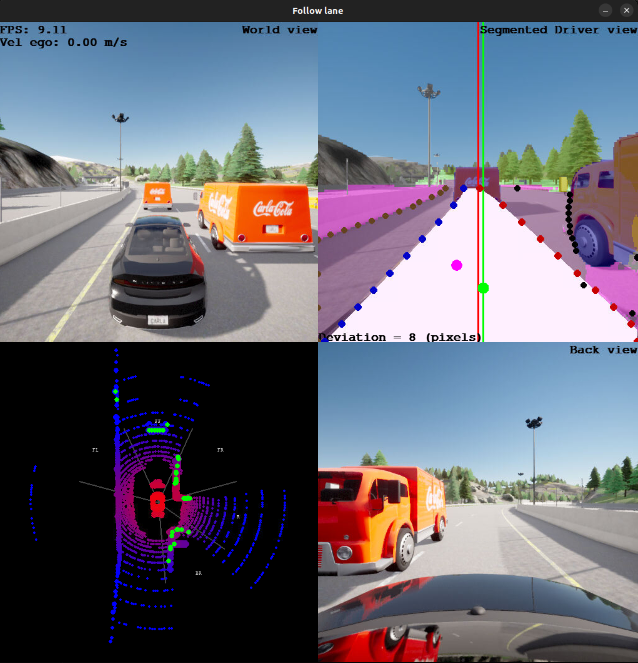
\includegraphics[width=9cm]{figs/Diseño/overtaken/obs.png}
\caption{Observaciones que recibe el modelo de adelantamiento basado en \ac{PPO}.}
\label{fig:obs_overtaken}
\end{figure}

El circuito usado durante todos los entrenamientos dispone de tres rutas en las que el coche va por el carril más a la derecha en una de ellas y, en las otras dos, por los carriles centrales. Para fomentar la visualización de todos los posibles estados en la calzada, se ha añadido una nueva ruta en la que el vehículo autónomo circula por el carril más a la izquierda, como se observa en la Figura \ref{fig:obs_overtaken}.

Como hemos visto en la definición de las observaciones, es necesario analizar todas las subzonas del \ac{LiDAR}, excluyendo la del lado izquierdo, para determinar cuándo es seguro regresar al carril inicial durante el adelantamiento. Para intentar tener en cuenta solo información que concierne a la conducción, se ha realizado un filtrado por distancia dependiendo de la subzona, ya que, por ejemplo, necesitamos más rango en la zona frontal del \ac{LiDAR} que en la lateral. De esta manera, nos aseguramos que el modelo recibe solo puntos dentro de la carretera. Los filtros de distancia aplicados según la subzona son los siguientes:
\begin{itemize}
\item \textit{Front}: no aplicamos filtro distancia, por lo que disponemos del rango total del \ac{LiDAR} (20 metros), como se muestra en la Figura \ref{fig:laser_front}.
\item \textit{Right-front}: nos quedamos con distancias iguales o menores a 7 metros.
\item \textit{Right}: filtrado por distancia de 6 metros.
\item \textit{Right-back}: se tienen en cuenta distancias inferiores a 9 metros.
\end{itemize}

\begin{figure}[ht]
\centering
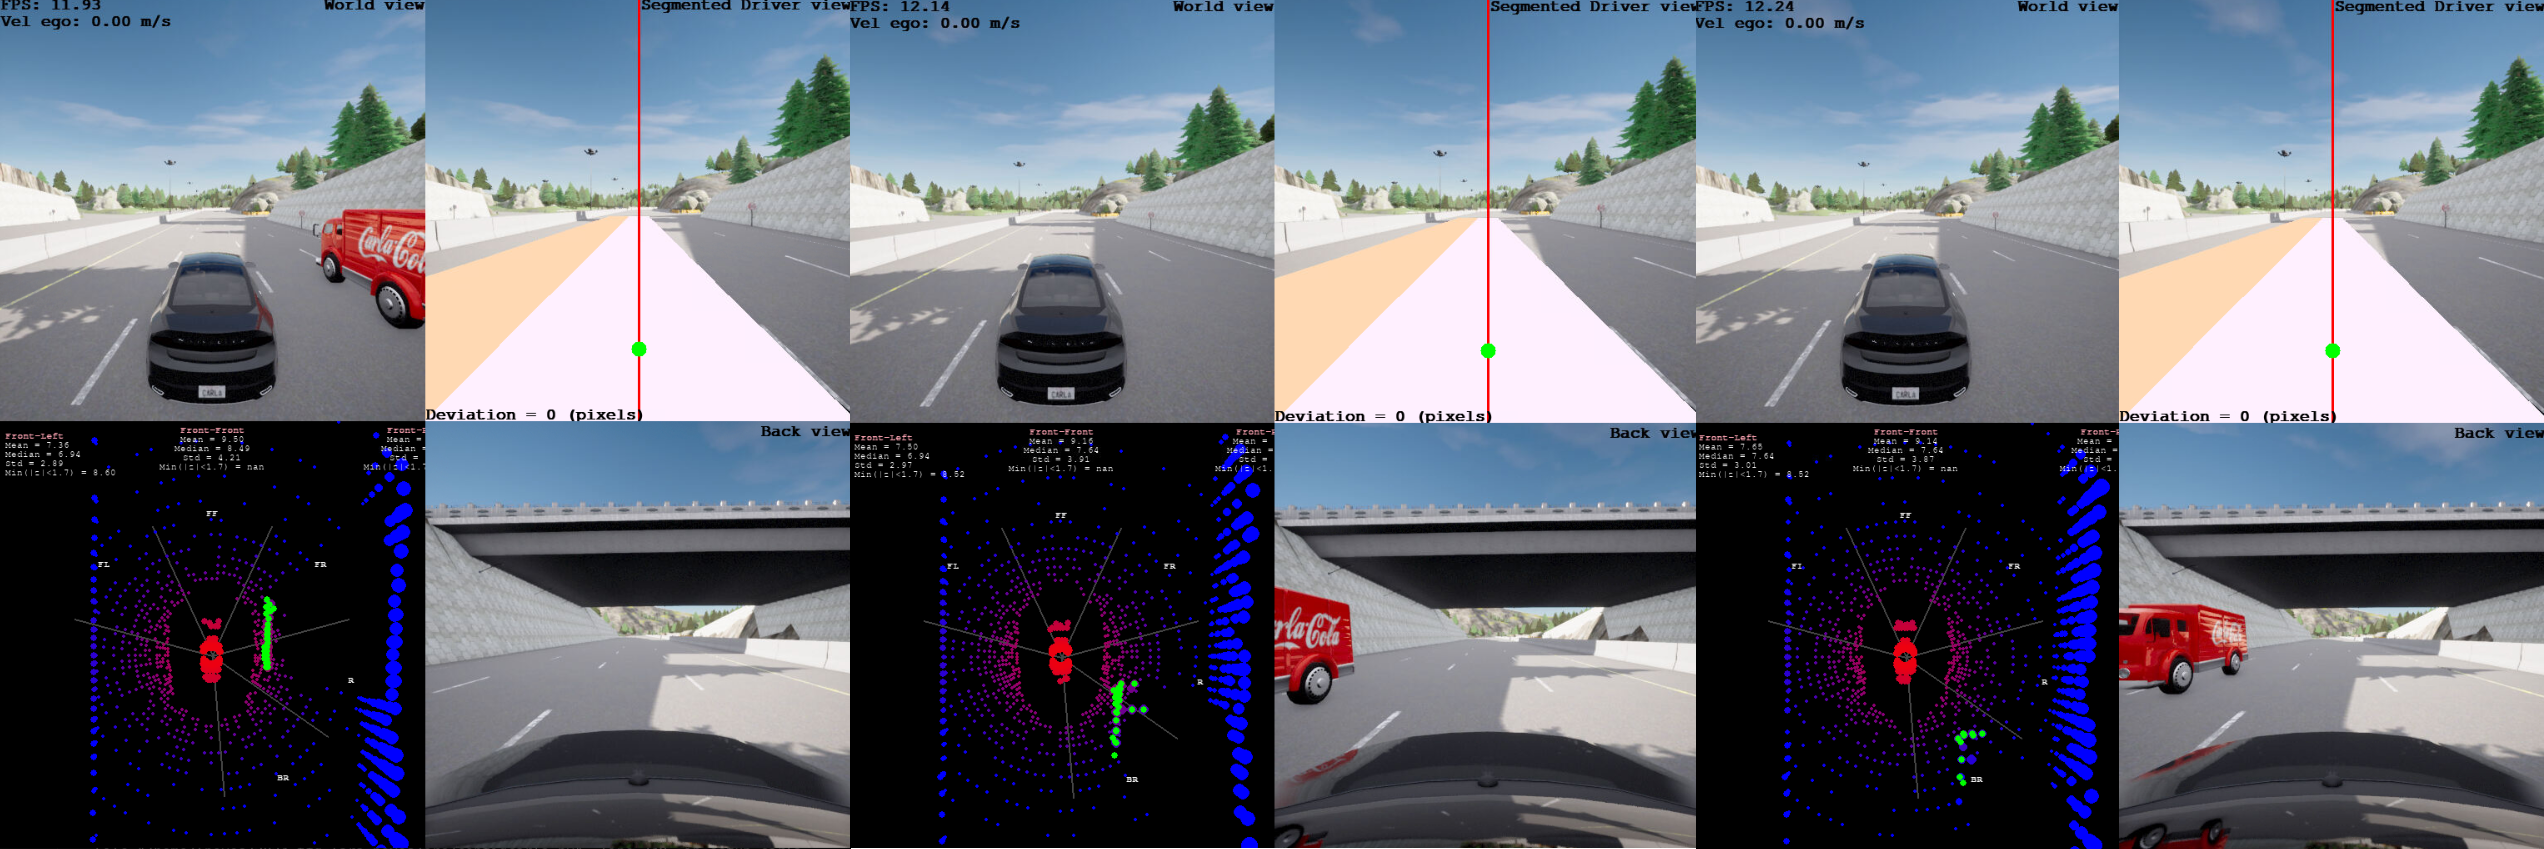
\includegraphics[width=\textwidth]{figs/Diseño/lidar/laser_right.png}
\caption{Filtrado por distancia del \ac{LiDAR} zona derecha.}
\label{fig:laser_right}
\end{figure}

Al igual que para el control de crucero adaptativo basado en \ac{PPO}, se ha empleado la estrategia de \textit{curriculum learning} \cite{curriculum-learning}, primero se ha entrenado un modelo capaz de seguir el carril de manera precisa con las nuevas observaciones. Sin embargo, debido al incremento significativamente en la cantidad de datos que recibe el modelo en comparación con comportamientos anteriores, el conjunto de observaciones se vuelve más complejo, ralentizando la convergencia y haciendo más difícil la obtención de soluciones óptimas. Por esta razón, se ha tenido que modificar la función de recompensa del sigue-carril, volviendo a la distinción entre acelerador bajo [0.0, 0.5) y moderado [0.5, 0.6). Además, en esta ocasión se ha incrementado el peso de la desviación y reducido el del acelerador respecto al modelo sigue-carril basado en \ac{PPO}, descrito en el código \ref{cod:rew_ppo}, dado que la presencia de mayor ruido dificulta el seguimiento del carril, y más a altas velocidades, es fundamental reforzar aún más la precisión para evitar que el modelo se vuelva inestable.

\begin{code}[h]
\begin{lstlisting}[language=Python]
elif self._throttle < 0.5:  # Low throttle
    w_dev, w_throttle, w_steer = 0.7, 0.2, 0.1
else:  # High throttle
    w_dev, w_throttle, w_steer = 0.75, 0.05, 0.2
\end{lstlisting}
\caption[Función de recompensa sigue-carril para el adelantamiento basado en \ac{PPO}]{Función de recompensa sigue-carril para el adelantamiento basado en \ac{PPO}.}
\label{cod:rew_ppo_lane_overtaken}
\end{code}

\newpage

Se ha ajustado la frecuencia de ejecución de CARLA a 5 \ac{FPS}, ya que en inferencia se logra alcanzar como máximo unos 10 \ac{FPS}. De este modo, garantizamos que podemos probar los modelos incluso cuando haya otros programas o entrenamientos en curso, puesto que el número de \ac{FPS} en inferencia siempre debe ser mayor al fijado en los entrenamientos con el modo síncrono de CARLA. No obstante, se han reutilizado los parámetros de seguimiento de carril basado en \ac{PPO}, detallados en la tabla \ref{tab:hiper_params_ppo}, exceptuando el coeficiente de entropía que, como también se hizo en el control de crucero adaptativo, se ha reducido a 0.08 para fomentar la explotación frente a la exploración. Los entrenamientos duraron aproximadamente entre cuatro y cinco días.

La Figura \ref{fig:train_lane_overtaken} muestra que el modelo finalmente converge, ya que 
se observa una tendencia ascendente en la recompensa media, que finalmente se estabiliza, y
en la gran mayoría de los episodios se completa el recorrido, aunque existen algunas excepciones, en contraste con el entrenamiento previo del sigue-carril basado en \ac{PPO}, reflejado en la Figura \ref{fig:train_ppo_carril}, donde no ocurrían estos fallos. Esto se debe a que el agente se ve afectado por la información innecesaria en las observaciones (\ac{LiDAR} y segmentación de la calzada), dando lugar a episodios más caóticos y un aprendizaje menos estable.

\begin{figure}[ht]
\centering
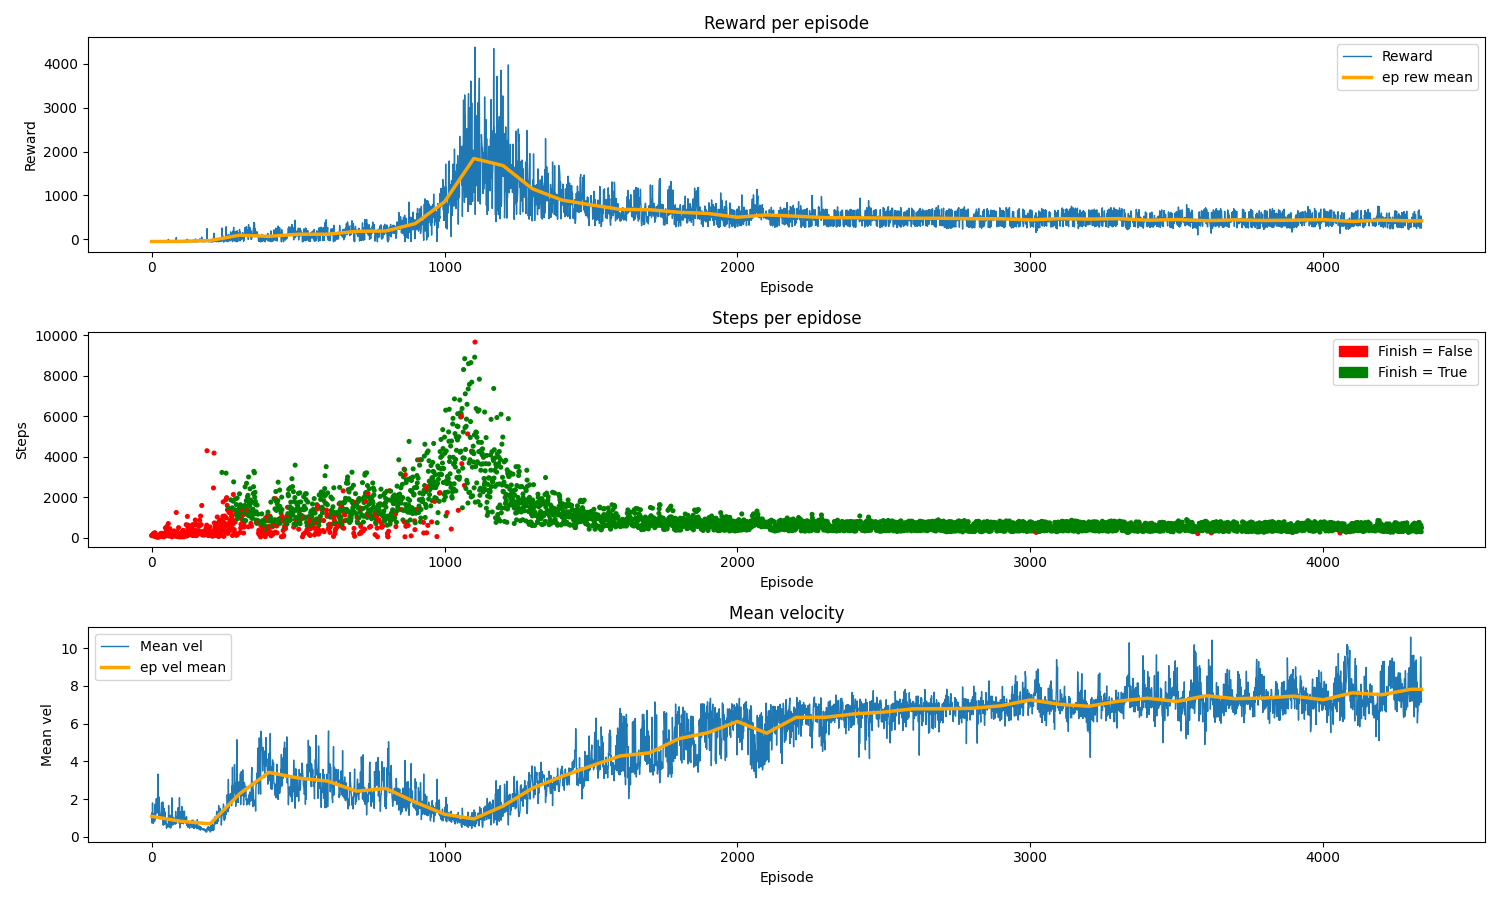
\includegraphics[width=14cm]{figs/Diseño/overtaken/train_lane.png}
\caption{Datos del entrenamiento sigue-carril para el adelantamiento basado en \ac{PPO}.}
\label{fig:train_lane_overtaken}
\end{figure}

Al igual que en los modelos anteriores de seguimiento de carril basados en \ac{PPO}, este modelo aprende que las acciones más óptimas son valores del acelerador moderados y giros sutiles. Similar al control de crucero adaptativo, obtenemos velocidades ligeramente inferiores a las del modelo exclusivo de seguimiento de carril debido al ruido introducido por las observaciones del \ac{LiDAR} y EfficientVit, que no son relevantes para esta tarea, y el aumento de la latencia total del sistema. Aun así, en inferencia logramos alcanzar velocidades de 40 km/h y un seguimiento de carril fluido y preciso\footnote{\url{https://youtu.be/KbqZBtF94Zg?si=ZCgzfXDVZrmrB-cF}}.
\begin{figure}[ht]
\centering
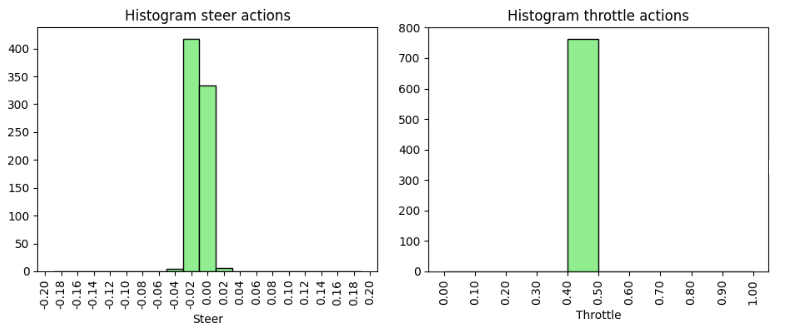
\includegraphics[width=13cm]{figs/Diseño/overtaken/inference_lane.png}
\caption{Datos en inferencia del sigue-carril para el adelantamiento basado en \ac{PPO}.}
\label{fig:inference_lane_overtaken}
\end{figure}

Una vez el coche ha logrado seguir el carril con precisión, debemos definir el escenario donde llevaremos a cabo el adelantamiento. Para ello, es necesario construir una máquina de estados que nos permita modificar la recompensa según la fase del adelantamiento en que esté el agente. Este proceso se describe en la Figura \ref{fig:dim _overtaken}.
\begin{figure}[ht]
\centering
\includegraphics[width=15cm]{figs/Diseño/overtaken/diagrama.jpg}
\caption{Diagrama de las fases del adelantamiento.}
\label{fig:dim _overtaken}
\end{figure}

\begin{enumerate}
\item \textit{Inicio del adelantamiento: sigue-carril.} El agente circula por su carril hasta que detecta con el \ac{LiDAR} al vehículo que circula delante suyo (alcance de 20 metros). Durante este tramo, recibe la recompensa referente al seguimiento de carril, especificada en el código \ref{cod:rew_ppo_lane_overtaken}.
\item \textit{Cambio al carril izquierdo.} Una vez detectado el vehículo delantero, se inicia la maniobra de adelantamiento y la recompensa cambia para incentivar al agente a cambiar al carril de la izquierda, si lo hay, lo cual se comprueba con la red de segmentación EfficientVit. Si el vehículo delantero deja de ser percibido, se interrumpe el adelantamiento y se vuelve al modo sigue-carril.
\item \textit{Adelantamiento: sigue-carril.} Una vez el agente está en el carril izquierdo, se retoma la recompensa del seguimiento de carril hasta que el agente detecta con el \ac{LiDAR} que ha sobrepasado al otro vehículo y que es seguro volver al carril inicial.
\item \textit{Vuelta al carril inicial.} En este momento, la función de recompensa cambia para que el modelo aprenda que debe desplazarse al carril de la derecha.
\item \textit{Fin del adelantamiento: sigue-carril.} Una vez realizado el cambio de carril, la maniobra de adelantamiento ha finalizado y se reanuda la recompensa sigue-carril hasta finalizar el recorrido.
\end{enumerate}

Para diseñar las recompensas para los cambios de carril, hemos modificado la normalización de la desviación, permitiendo al modelo que aprenda de manera eficiente sin necesidad de indicaciones explícitas sobre cuándo y con qué magnitud realizar el giro, solamente especificamos en qué dirección debe moverse. Si queremos que el agente se desplace al carril de la izquierda, lo cual supone una desviación positiva, cuanto mayor sea la desviación, mayor será la recompensa. Si la desviación es negativa, el valor de la recompensa será cero. Por el contrario, si el objetivo es volver al carril de la derecha, cuanto más negativa sea la desviación, mayor será la recompensa. Si la desviación es positiva, la recompensa es nula. Una vez normalizada la desviación, aplicamos la función \textit{sigmoide}, expuesta en la Figura \ref{fig:sigmoide}, para acentuar la diferencia entre grandes desviaciones y aquellas más centradas. Esto permite al modelo aprender más rápido cuáles son las acciones óptimas. 

  \begin{myequation}[H]
    \begin{equation} 
       r_{\text{dev}} = \frac{1}{1 + e^{-a \cdot (dev_{\text{norm}} - b)}}
    \end{equation} 
    \caption{Fórmula de la función \textit{sigmoide}.}
\label{eq:sigmoid_deviation}
  \end{myequation}

\begin{figure}[ht]
\centering
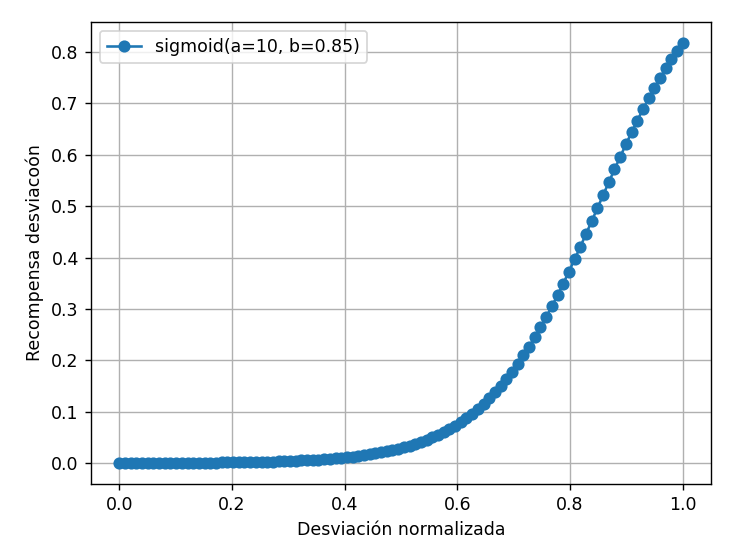
\includegraphics[width=7cm]{figs/Diseño/overtaken/sigmoide.png}
\caption{Función \textit{sigmoide} aplicada a la desviación para el cambio de carril.}
\label{fig:sigmoide}
\end{figure}

\newpage

En el caso del cambio de carril a la izquierda, también se tiene en cuenta el valor del \ac{LiDAR} en la recompensa para realizar una maniobra más segura, evitando que el agente se aproxime demasiado al vehículo delantero o incluso colisione contra él, como se observa en la Figura \ref{fig:esquema_over}. Tanto si se choca con el vehículo, como si se sale o cambia de carril de manera incorrecta, es decir, cuando no debe o hacia el lado equivocado, el episodio se finaliza con una recompensa negativa.
\begin{figure}[ht]
\centering
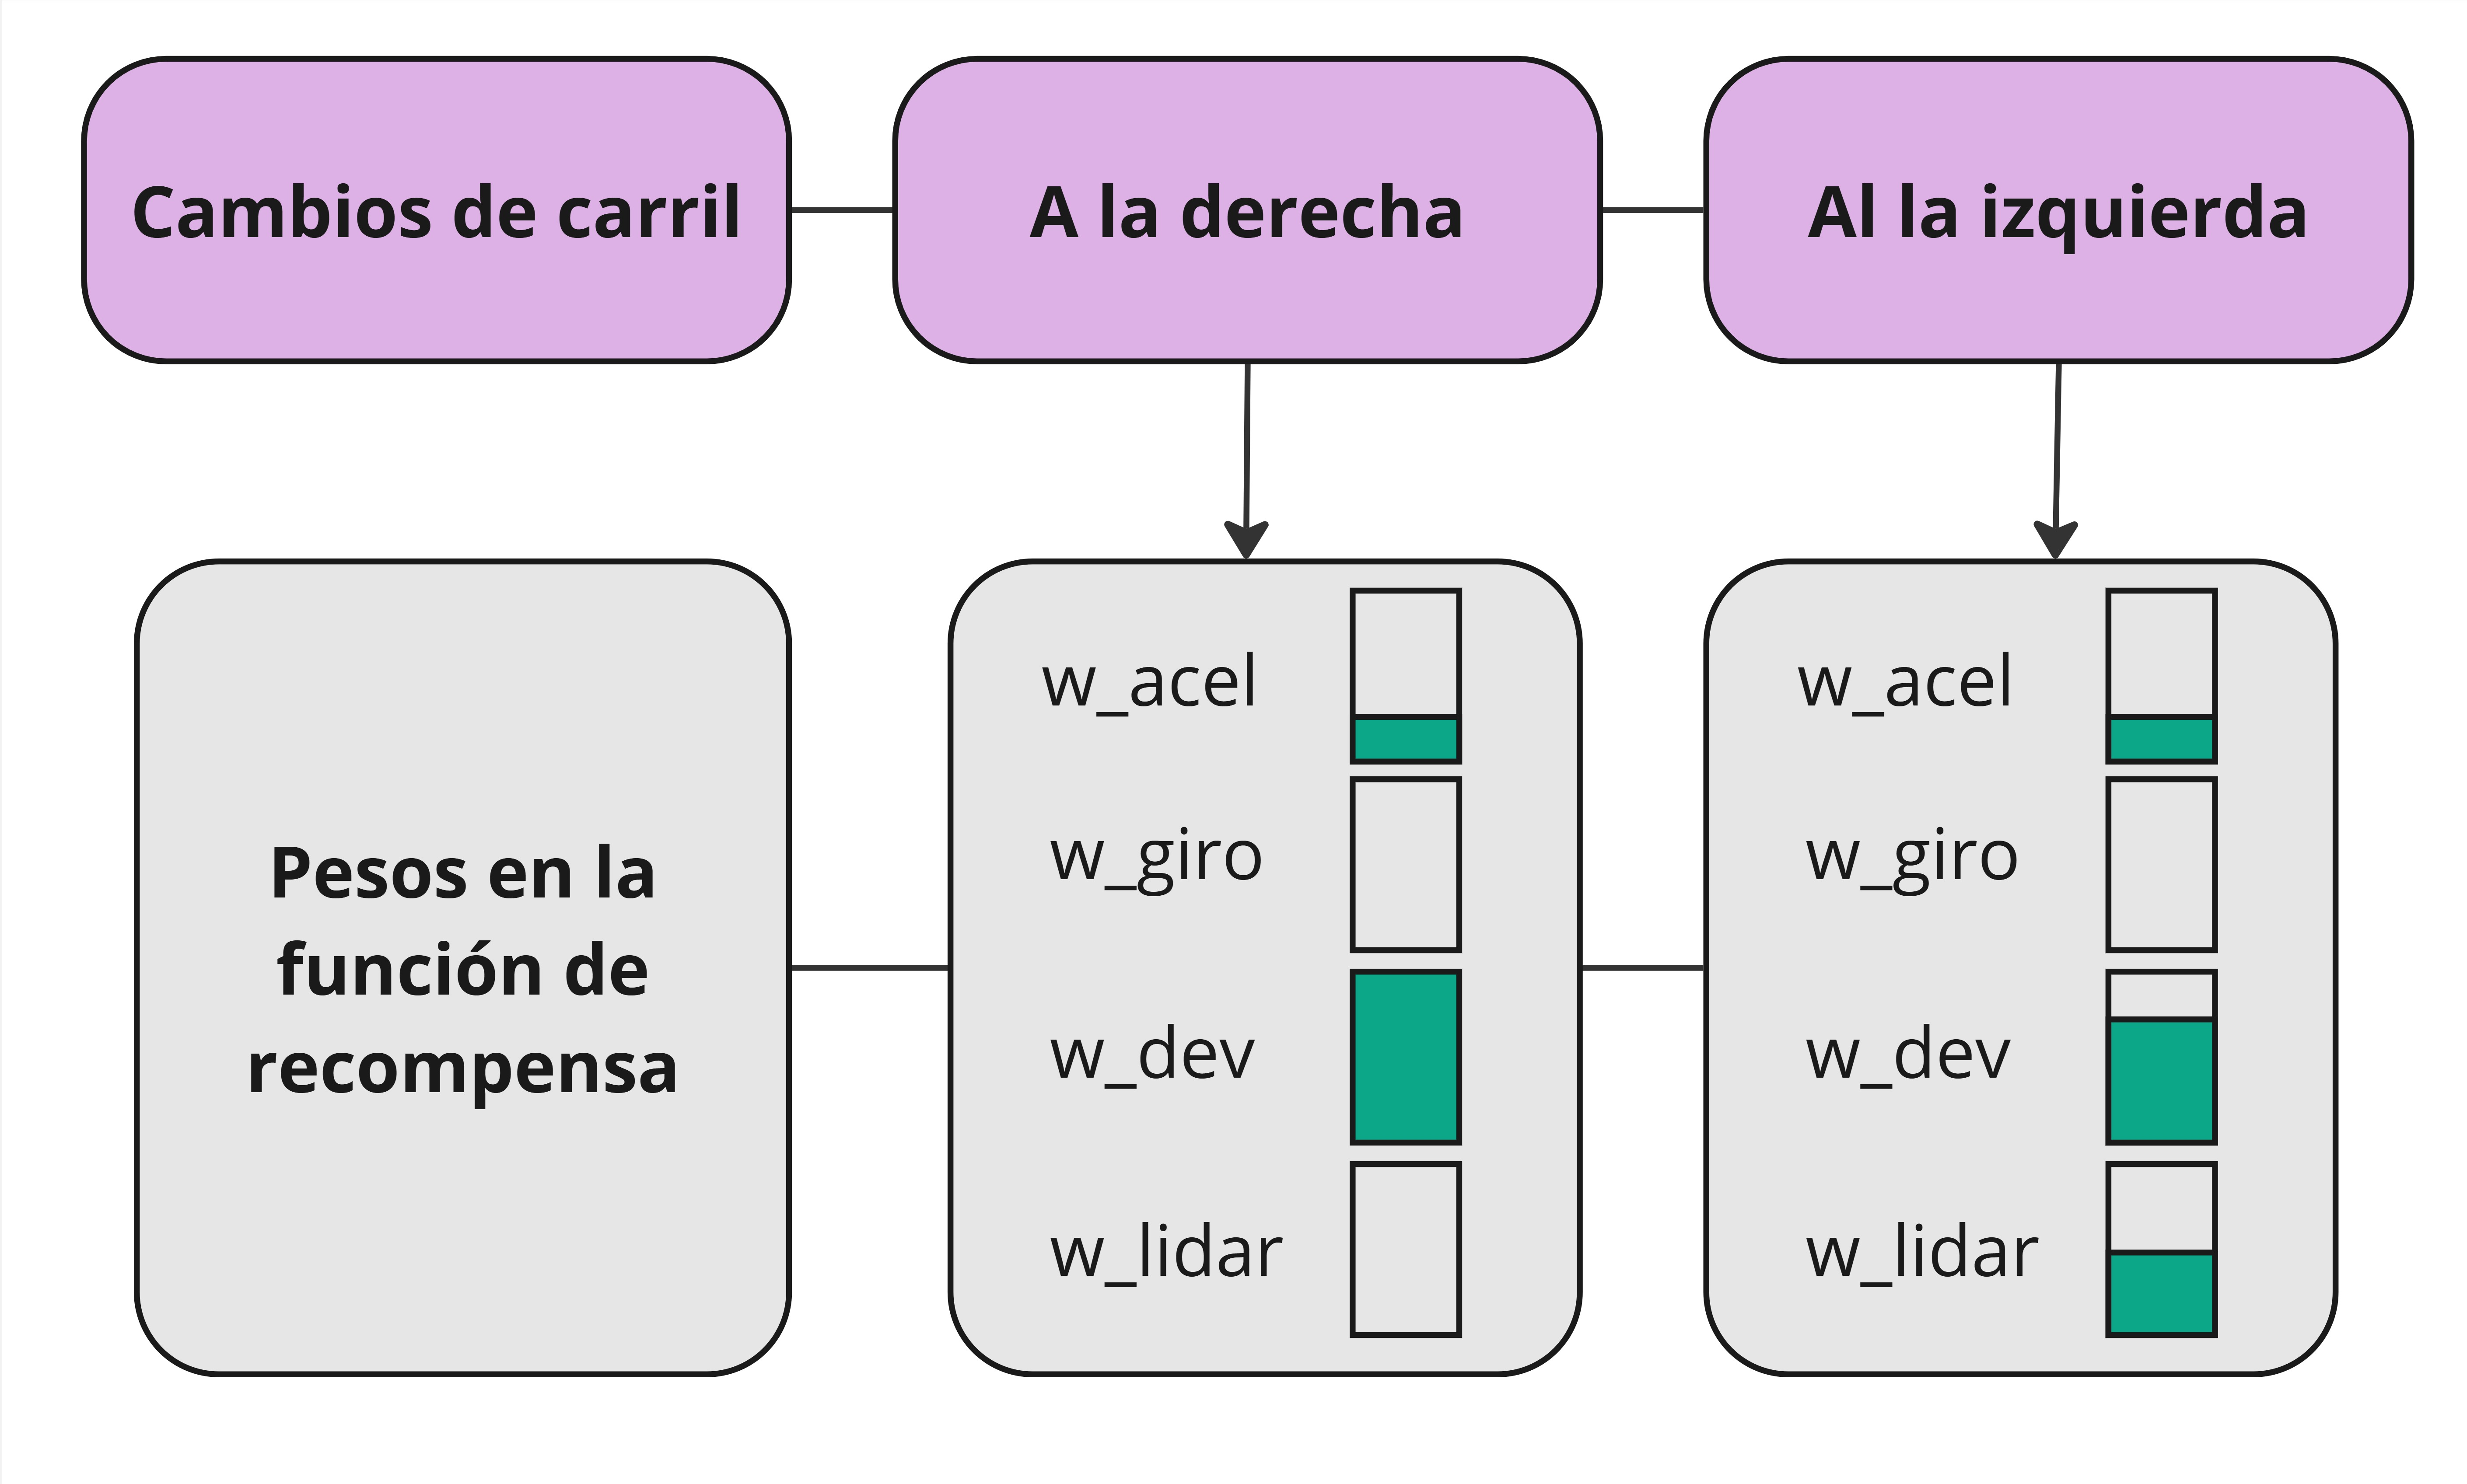
\includegraphics[width=10cm]{figs/Diseño/overtaken/esquema.jpg}
\caption{Esquema de recompensa para el adelantamiento basado en \ac{PPO}.}
\label{fig:esquema_over}
\end{figure}

\begin{code}[H]
\begin{lstlisting}[language=Python]
if error == None:
    # Deviation normalization
    if self._overtaken_in_progress and left_lane:
        # Positive deviation
        dev_norm = np.clip(self._dev, 0, MAX_DEV_CHANGE) / MAX_DEV_CHANGE
        r_dev = sigmoid(dev_norm, a=10, b=0.85)
    elif self._overtaken_in_progress and right_lane:
        # Negative deviation 
        dev_norm = abs(np.clip(self._dev, -MAX_DEV_CHANGE, 0)) / MAX_DEV_CHANGE
        r_dev = sigmoid(dev_norm, a=10, b=0.85)
    else:
        r_dev =  (MAX_DEV - abs(np.clip(self._dev, -MAX_DEV, MAX_DEV))) / MAX_DEV

    # Steer, throttle and LiDAR conversion

    # Set weights
    # Filter inadequate actions
    elif self._velocity > self._max_vel:
        if not self._overtaken_in_progress:
            w_dev, w_throttle, w_steer, w_lidar = 0.1, 0.65, 0.25, 0.0
        else:
            w_dev, w_throttle, w_steer, w_lidar = 0.4, 0.6, 0.0, 0.0
    elif self._overtaken_in_progress and left_lane:
        w_dev, w_throttle, w_steer, w_lidar = 0.65, 0.1, 0.0, 0.25
    elif self._overtaken_in_progress and right_lane:
        w_dev, w_throttle, w_steer, w_lidar = 0.85, 0.15, 0.0, 0.0  
    # Follow lane

    reward = w_dev * r_dev + w_throttle * r_throttle + w_steer * r_steer + w_laser * r_lidar
else:
    if "crashed" in error:
        reward = -60  # Crashed into the vehicle in front
    else:
        reward = -40  # Lane lost
\end{lstlisting}
\caption[Función de recompensa para el adelantamiento basado en \ac{PPO}]{Función de recompensa para el adelantamiento basado en \ac{PPO}.}
\label{cod:rew_ppo_overtaken}
\end{code}

El entrenamiento se ha llevado a cabo en un circuito con cuatro carriles, donde nuestro coche circula por el carril central izquierdo. El vehículo delantero comienza a una distancia aleatoria de 20 a 40 metros del agente y mantiene una velocidad constante de 5 m/s durante todo el recorrido. Sin embargo, para evitar perderlo de vista, si se aleja a más de 25 metros del agente se detiene. Al igual que en el reentrenamiento de control de crucero adaptativo, disminuimos el coeficiente de entropía a 0.04 para acelerar el entrenamiento evitando escenarios infrecuentes. Los entrenamientos tuvieron una duración de aproximadamente dos días, con un total de dos millones de \textit{steps}.

En la Figura \ref{fig:train_overtaken}, se presentan los datos recopilados durante el entrenamiento. Los resultados muestran una mejora progresiva en la recompensa, indicando que el agente ha aprendido a realizar la maniobra de adelantamiento. Sin embargo, se observan fluctuaciones significativas en la recompensa, referentes a los episodios no finalizados, sugiriendo que la política aún no es completamente estable y que el modelo no ha alcanzado una convergencia total. Para mejorar la estabilidad y reducir la frecuencia de episodios fallidos, sería necesario aumentar el tiempo de entrenamiento.
\begin{figure}[ht]
\centering
\includegraphics[width=\textwidth]{figs/Diseño/overtaken/train.png}
\caption{Datos del reentrenamiento para el modelo de adelantamiento basado en \ac{PPO}.}
\label{fig:train_overtaken}
\end{figure}

Durante la fase de inferencia, en el circuito de entrenamiento con el vehículo delantero a 4 m/s\footnote{\url{https://youtu.be/MOkeUKRlw9o}}, el agente es capaz de ejecutar la maniobra de adelantamiento de manera segura, sin ponerse en riesgo ni a sí mismo ni al otro vehículo en la vía. Sin embargo, aún presenta cierto grado de descontrol, demostrando de nuevo que aún se requiere más tiempo de entrenamiento para lograr una solución más óptima y precisa. Además, sería posible incrementar la velocidad durante el adelantamiento, dado que, a medida que el agente mejora su precisión y estabilidad, tiende a aumentar su velocidad, como se observó en los modelos de seguimiento de carril.

Como se muestra en la Figura \ref{fig:inference_overtaken}, los valores del acelerador se mantienen similares a los obtenidos en el modelo base de seguimiento de carril (ver Figura \ref{fig:inference_lane_overtaken}). Por otro lado, el giro sigue estando mayoritariamente centrado, puesto que en la gran parte del circuito el agente realiza un comportamiento de sigue-carril. Sin embargo, se observa la aparición de giros más pronunciados, utilizados para llevar a cabo tanto el cambio de carril a la izquierda como a la derecha.

\begin{figure}[ht]
\centering
\includegraphics[width=\textwidth]{figs/Diseño/overtaken/inference.png}
\caption{Acciones escogidas en inferencia durante adelantamiento basado en \ac{PPO}.}
\label{fig:inference_overtaken}
\end{figure}
\newpage

Al introducir la red neuronal EfficientVit y su post-procesado para la segmentación de la calzada, la latencia aumenta drásticamente en más de 50 ms. Como vimos en el apartado de percepción \ref{fig:profiling}, estas operaciones son de las más costosas en términos computacionales. Aunque contamos con un modelo más complejo, que considera una mayor cantidad de información para la toma de decisiones, el incremento en la latencia respecto a los modelos anteriores basados en \ac{PPO} es mínimo. Finalmente, el sistema alcanza una latencia total de 86 ms, permitiéndole ejecutar a unos 11-12 \ac{FPS} en el servidor Thor, mientras que CARLA  es capaz de ejecutar a 9-10 \ac{FPS}. A pesar de este decremento en la velocidad de ejecución, el sistema sigue siendo válido para aplicaciones en tiempo real.
\begin{figure}[ht]
\centering
\includegraphics[width=14cm]{figs/Diseño/overtaken/profiling.png}
\caption{\textit{Profiling} del modelo de adelantamiento basado en \ac{PPO}.}
\label{fig:profiling_overtaken}
\end{figure}

